%=================================================================
\documentclass[Universe,article,submit,moreauthors,pdftex]{Definitions/mdpi} 
%=================================================================
\firstpage{1} 
\makeatletter 
\setcounter{page}{\@firstpage} 
\makeatother
\pubvolume{xx}
\issuenum{1}
\articlenumber{5}
\pubyear{2020}
\copyrightyear{2020}
%\externaleditor{Academic Editor: Roman Pasechnik}

%\preto{\abstractkeywords}{\nolinenumbers} %>>>>nolinenumbers<<<
%\history{Received: 10 September 2020; Accepted: date; Published: date}
%\updates{yes} % If there is an update available, un-comment this line

%% MDPI internal command: uncomment if new journal that already uses continuous page numbers 
%\continuouspages{yes}

%------------------------------------------------------------------
% The following line should be uncommented if the LaTeX file is uploaded to arXiv.org
\pdfoutput=1

%=================================================================
% Add packages and commands here. The following packages are loaded in our class file: fontenc, inputenc, calc, indentfirst, fancyhdr, graphicx,epstopdf, lastpage, ifthen, lineno, float, amsmath, setspace, enumitem, mathpazo, booktabs, titlesec, etoolbox, tabto, xcolor, soul, multirow, microtype, tikz, totcount, amsthm, hyphenat, natbib, hyperref, footmisc, url, geometry, newfloat, caption
\usepackage{xcolor}
\usepackage{graphicx}
\usepackage{amsmath}
\usepackage{amssymb}
\usepackage{epstopdf}
\usepackage{comment}

\newcommand{\beqn}{\begin{equation}}
\newcommand{\eeqn}{\end{equation}}
\newcommand{\req}[1]{Eq.\,(\ref{#1})}
\newcommand{\TeV}{\text{ TeV}}
\newcommand{\GeV}{\text{ GeV}}
\newcommand{\MeV}{\text{ MeV}}
\newcommand{\keV}{\text{ keV}}
\newcommand{\eV}{\text{ eV}}
\newcommand{\meV}{\text{ meV}}
%\newcommand*{\req}[1]{Eq.~{\eqref{#1}}}
\newcommand*{\rf}[1]{Fig.~{\ref{#1}}}
\newcommand*{\rsec}[1]{Sect.\,{\ref{#1}}}
\newcommand*{\bb}{\boldsymbol}
\newcommand*{\xred}{\color{red}}
\newcommand*{\xblue}{\color{blue}}
\newcommand*{\xgreen}{\color{green}}

%=================================================================
%% Please use the following mathematics environments: Theorem, Lemma, Corollary, Proposition, Characterization, Property, Problem, Example, ExamplesandDefinitions, Hypothesis, Remark, Definition, Notation, Assumption
%% For proofs, please use the proof environment (the amsthm package is loaded by the MDPI class).

%=================================================================
% Full title of the paper (Capitalized)
\Title{\uppercase{A Short Survey of Matter-Antimatter Evolution in the Primordial Universe}}

% Author Orcid ID: enter ID or remove command
\newcommand{\orcidauthorA}{0000-0001-8217-1484} % Add \orcidA{} behind the author's name
\newcommand{\orcidauthorB}{0000-0001-5038-8427} % Add \orcidB{} behind the author's name
\newcommand{\orcidauthorC}{0000-0001-5474-2649} % Add \orcidC{} behind the author's name
\newcommand{\orcidauthorD}{0000-0002-2289-4856}
 
% Authors, for the paper (add full first names)
\Author{Johann Rafelski\orcidA{}, Jeremiah Birrell\orcidD, Andrew Steinmetz\orcidC{}, and Cheng Tao Yang\orcidB{}}
% Authors, for metadata in PDF
\AuthorNames{Johann Rafelski, Jeremiah Birrell, Andrew Steinmetz, and Cheng Tao Yang}

% Affiliations / Addresses (Add [1] after \address if there is only one affiliation.)
\address[1]{%
Department of Physics, The University of Arizona, Tucson, Arizona 85721, USA} 

% Contact information of the corresponding author
\corres{Correspondence: JohannR@arizona.edu
%; %Tel.: (optional; include country code; if there are multiple corresponding authors, add author initials) +xx-xxxx-xxx-xxxx (F.L.)
}

% Current address and/or shared authorship
%\firstnote{Current address: Affiliation 3} 
%\secondnote{These authors contributed equally to this work.}
% The commands \thirdnote{} till \eighthnote{} are available for further notes

%\simplesumm{} % Simple summary

%\conference{} % An extended version of a conference paper

% Abstract (Do not insert blank lines, i.e. \\) 

\abstract{We will write abstract here}
%
\keyword{Magnetization; Electron-Positron plasma; Cosmology.}
%%%%%%%%%%%%%%%%%%%%%%%%%%%%%%%%%%%%%%%
\begin{document}
%%%%%%%%%%%%%%%%%%%%%%%%%%%%%%%%%%%%%%% 
\section{Introduction}\label{sec:Intro}
\noindent In celebration of Remo Ruffini's 80th birthday and his contributions to astrophysics and cosmology, we offer here a survey of the matter-antimatter evolution of the primordial universe beginning with quark-gluon plasma (QGP) at a temperature of $130\GeV$ and ending with the electron-positron $e^{\pm}$ epoch which was the final phase of the universe to contain significant quantities of antimatter. This final cosmic soup of antimatter survived until the universe cooled to a temperature of $20\keV$. This work presumes that in our casual domain, the universe is matter dominated.

We present an overview of particle families across all epochs in the universe, as a function of temperature and thus time, and demonstrating that most evolutionary processes in the primordial universe were adiabatic and conversed entropy content over time. We take this opportunity to enlarge in some detail our more recent work in special topics on: strangeness content, neutrino freezeout, the lingering of pions, and the magnetization of the electron-positron plasma during and around the time of Big Bang Nucleosynthesis (BBN). After briefly discussing the disappearance of muons and antimuons at $4.2\MeV$, we will in more detail describe electron and positron plasmas.

While the disappearance of baryonic matter is well described in the literature, it has not always been appreciated how late leptonic ($\bar{\mu}=\mu^{+}$ and $\bar{e}=e^{+}$) antimatter remains a significant presence in the universe's evolutionary history. We show that the $e^{\pm}$ epoch is a prime candidate to tackle up to here several unrelated cosmic mysteries such as early universe matter in-homogeneity, the origin of cosmic magnetic fields. We note that $e^{\pm}$ dynamics may also apply to gamma-ray burst (GRB) and magnetars in the contemporary universe today.

%%%%%%%%%%%%%%%%%%%%%%%%%%%%%%%%%%%%%%%
\begin{figure}[htbp]
  \centering  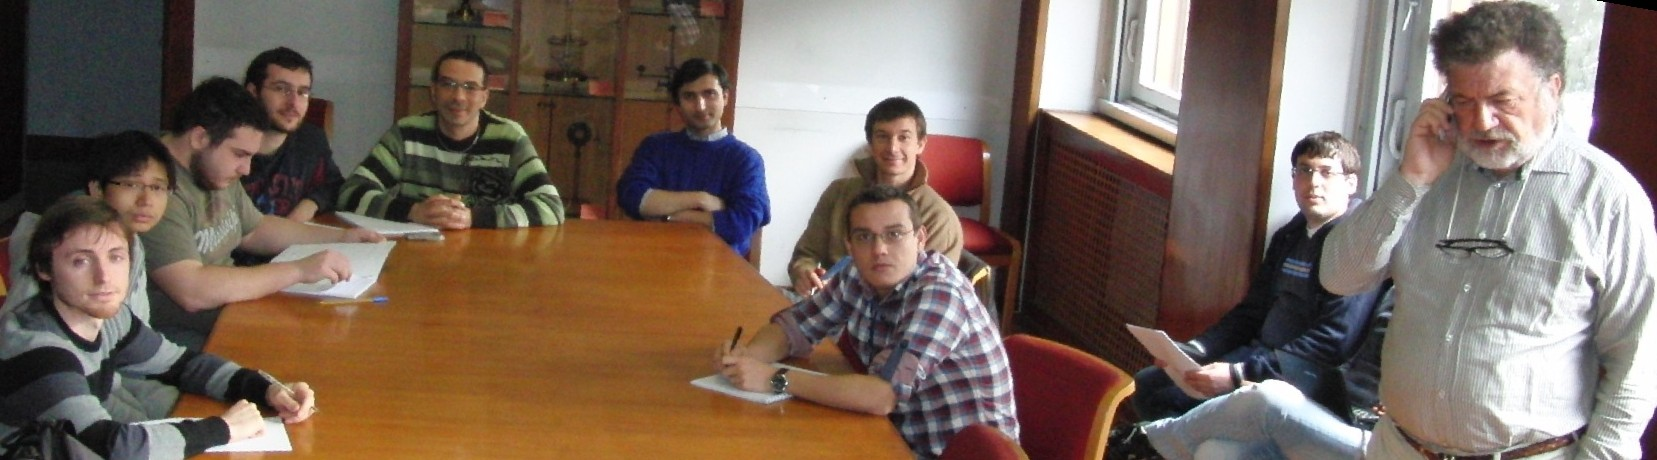
\includegraphics[width=\textwidth]{12MarchRemoAtWorkC.jpg}
  \label{RemoAtWork}
  \caption{Remo Ruffini (right) at work. Photo by Johann Rafelski.}
\end{figure}
%%%%%%%%%%%%%%%%%%%%%%%%%%%%%%%%%%%%%%%

\begin{itemize}
  \item {\xred Introducing the major topics of the paper. The \lq\lq five\rq\rq\ plasma epochs in the universe with some sub-epochs detailed and a brief dive into $e^{\pm}$ plasma as our bread and butter. First paragraph should emphasize the anti-matter of the early universe.}
  \item {\xred If the universe is symmetric in matter/antimatter, then the universe domain we reside in antimatter disappears as a major component at 20 keV.}
  \item {\xred This paper does NOT resolve matter/antimatter asymmetry, rather it explores the consequences of evolution once that asymmetry is already present.}
  \item {\xred We cutoff discussion at 20 keV as antimatter from the Big Bang has disappeared with the loss of the positrons. Antimatter is then only from secondary processes, and the matter universe (electron-proton) further cools resulting in recombination and the CMB. Then observational cosmology begins.}
  \item {\xred The electron-light nuclei domain is more the area of standard cosmology. It has not been appreciated that antimatter was so prevalent above 20 keV thus that is where our efforts reside.}
  \item {\xred 80th birthday is a good opportunity to remember Remo Ruffini's contribution to astrophysics and our mutual interest in the cosmic evolution of the universe. First paragraph is organizational. What's we're talking about and why. Add some RR references with explicitly electron-positron content, also note our work could potential be a model of GRB.}
  \item {\xred Section on neutrino oscillation, and mass models, and magnetic moments.}
  \item {\xred Note that in the early leptonic epoch, the ratios of energy densities is fixed by the number of species allowed which is why the order of energy density goes neutrino, electrons, then photons.}
\end{itemize}
%%%%%%%%%%%%%%%%%%%%%%%%%%%%%%%%%%%%%%%
\begin{figure} 
  \centerline{\hspace*{0.4cm}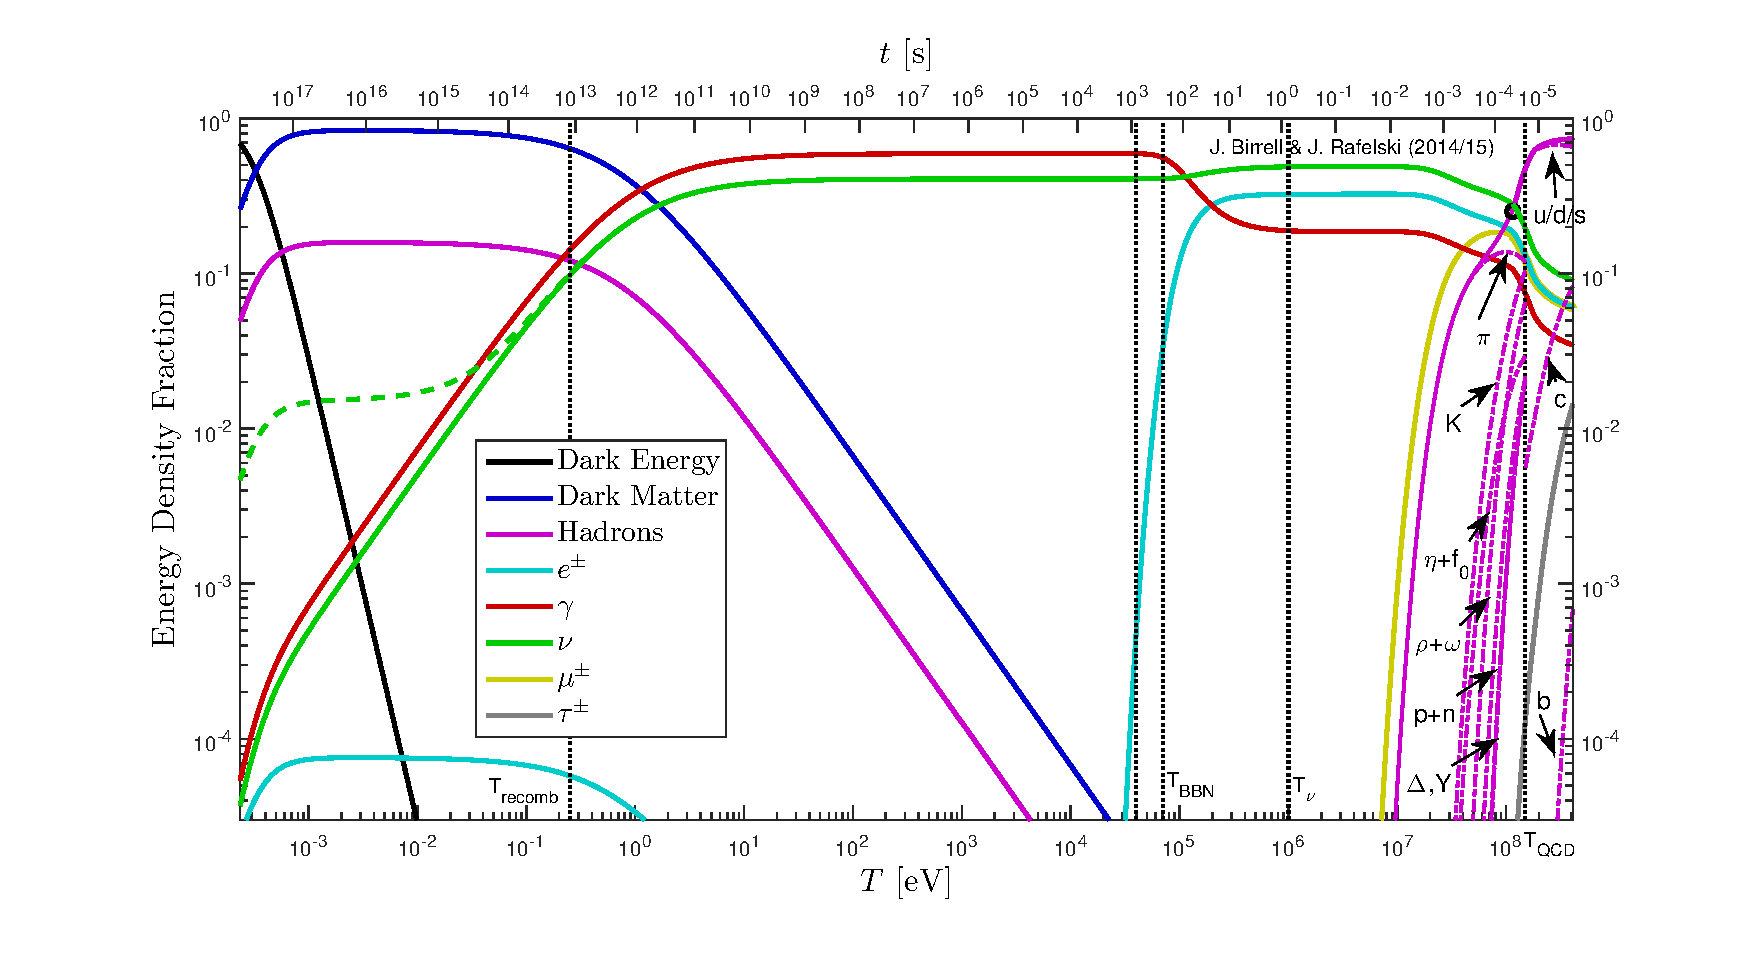
\includegraphics[height=11cm]{./plots/energy_fractions.eps}}
  \centerline{\hspace*{0.4cm}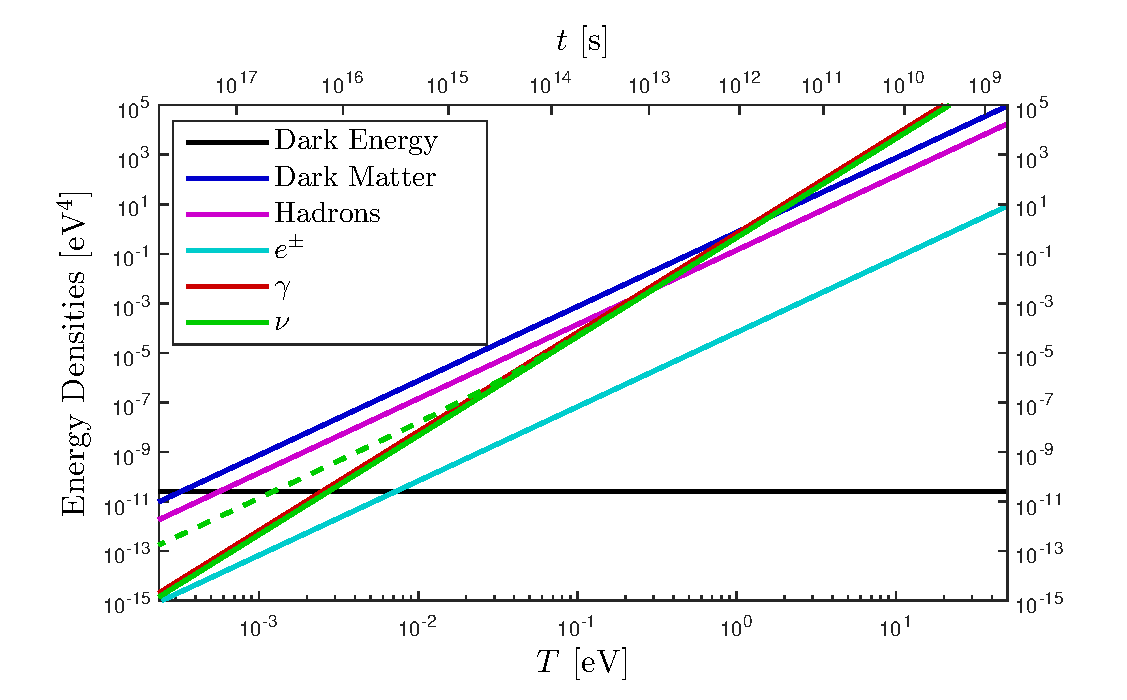
\includegraphics[height=8.5cm]{./plots/energy_densities.eps}}
  \caption{Current era: $69\%$ dark energy, $26\%$ dark matter, $5\%$ baryons, $<1\%$ photons and neutrinos.  Solid neutrino line shows massless neutrinos while the dashed line shows $1$ massless and $2\times 0.1$ eV neutrinos (Neutrino mass choice is just for illustration.  Other values are possible).\label{fig:energy_frac}}
   \end{figure}
%%%%%%%%%%%%%%%%%%%%%%%%%%%%%%%%%%%%%%%

\section{Timeline of particles and plasmas in the universe}\label{sec:Timeline}
\noindent At an early time in the standard cosmology model, the universe began as a fireball with extremely high temperature and high energy density. The ultra-relativistic plasma produced in the early universe contained almost a perfect symmetry between matter and antimatter except for a small discrepancy of one part in $10^{9}$ which remains a mystery today. This fireball then underwent several phases changes which dramatically evolved the gross properties as the universe expanded and cooled. The comic plasma, after the electroweak symmetry breaking epoch and presumabely inflation, occured in the early universe in the following sequence:
\begin{enumerate}
  \item \textbf{Primordial quark-gluon plasma}: At early times when the temperature was between $130\ \mathrm{GeV}>T>150\ \mathrm{MeV}$, we have the building blocks of universe as we know them today including the leptons, vector bosons, and all three families of de-confined quarks and gluons which propagated freely. As all hadrons are dissolved into their constituents during this time, strongly interacting particles $u,d,s,t,b,c,g$ controlled the fate of the universe. Here we will only look at the late-stage evolution at around $150\MeV$.
  \item \textbf{Hadronic epoch}: Around the hadronization temperature $T_h\approx150\ \mathrm{MeV}$, a phase transformation occured forcing the stongly interacting particles such as quarks and gluons to condense into confined states. It is here where matter as we know it today forms and the universe becomes hadronic-matter dominated. In the temperature range $ 60\ \mathrm{MeV}>T>20\ \mathrm{MeV}$ the universe is rich in physics phenomena involving strange mesons and (anti)baryons including (anti)hyperon abundances \cite{Fromerth:2012fe,Yang:2021bko}.
  \item  \textbf{Lepton-photon epoch}: For temperature $10\ \mathrm{MeV}>T>2\ \mathrm{MeV}$, the universe contained relativistic electrons, positrons, photons, and three species of neutrinos/antineutrinos. Muons vanish partway through this temperature scale. In this range, neutrinos were still coupled to the charged leptons via the weak interaction. \cite{Birrell:2012gg}. During this time the expansion of the universe is controlled by leptons and photons almost on equal footing.
  \item  \textbf{Final antimatter epoch}: After neutrinos decoupled and become free-streaming, referred to as neutrino freezeout, from the cosmic plasma at $T=2\ \mathrm{MeV}$, the cosmic plasma was dominated by electrons, positrons, and photons. We have shown in \cite{Chris:2023abc} that this plasma existed until $T\approx0.02\ \mathrm{MeV}$ such that BBN occurred within a rich electron-positron plasma. This is the last time the universe will host a significant fraction of its content in antimatter.
  \item \textbf{Moving towards matter dominated universe}: The final major plasma stage in the universe began after the annihilation of the majority of $e^{\pm}$ pairs leaving behind a residual amount of electrons determined by the baryon asymmetry in the universe and charge conservation. The universe was still opaque to photons at this point and remained so until the recombination period at $T\approx0.26\ \mathrm{eV}$ starting the era of observational cosmology with the CMB. This final epoch of the primordial universe will not be described in detail here, but is well covered in {\xred Add Ref!}
\end{enumerate}
\begin{itemize}
    \item {\xred Add Jeremey's material here which acts like a more detailed look at the bullet points above.}
\end{itemize}
%%%%%%%%%%%%%%%%%%%%%%%%%%%%%%%%%%%%%%%
\begin{figure}[h]
  %\begin{center}
  \centering
  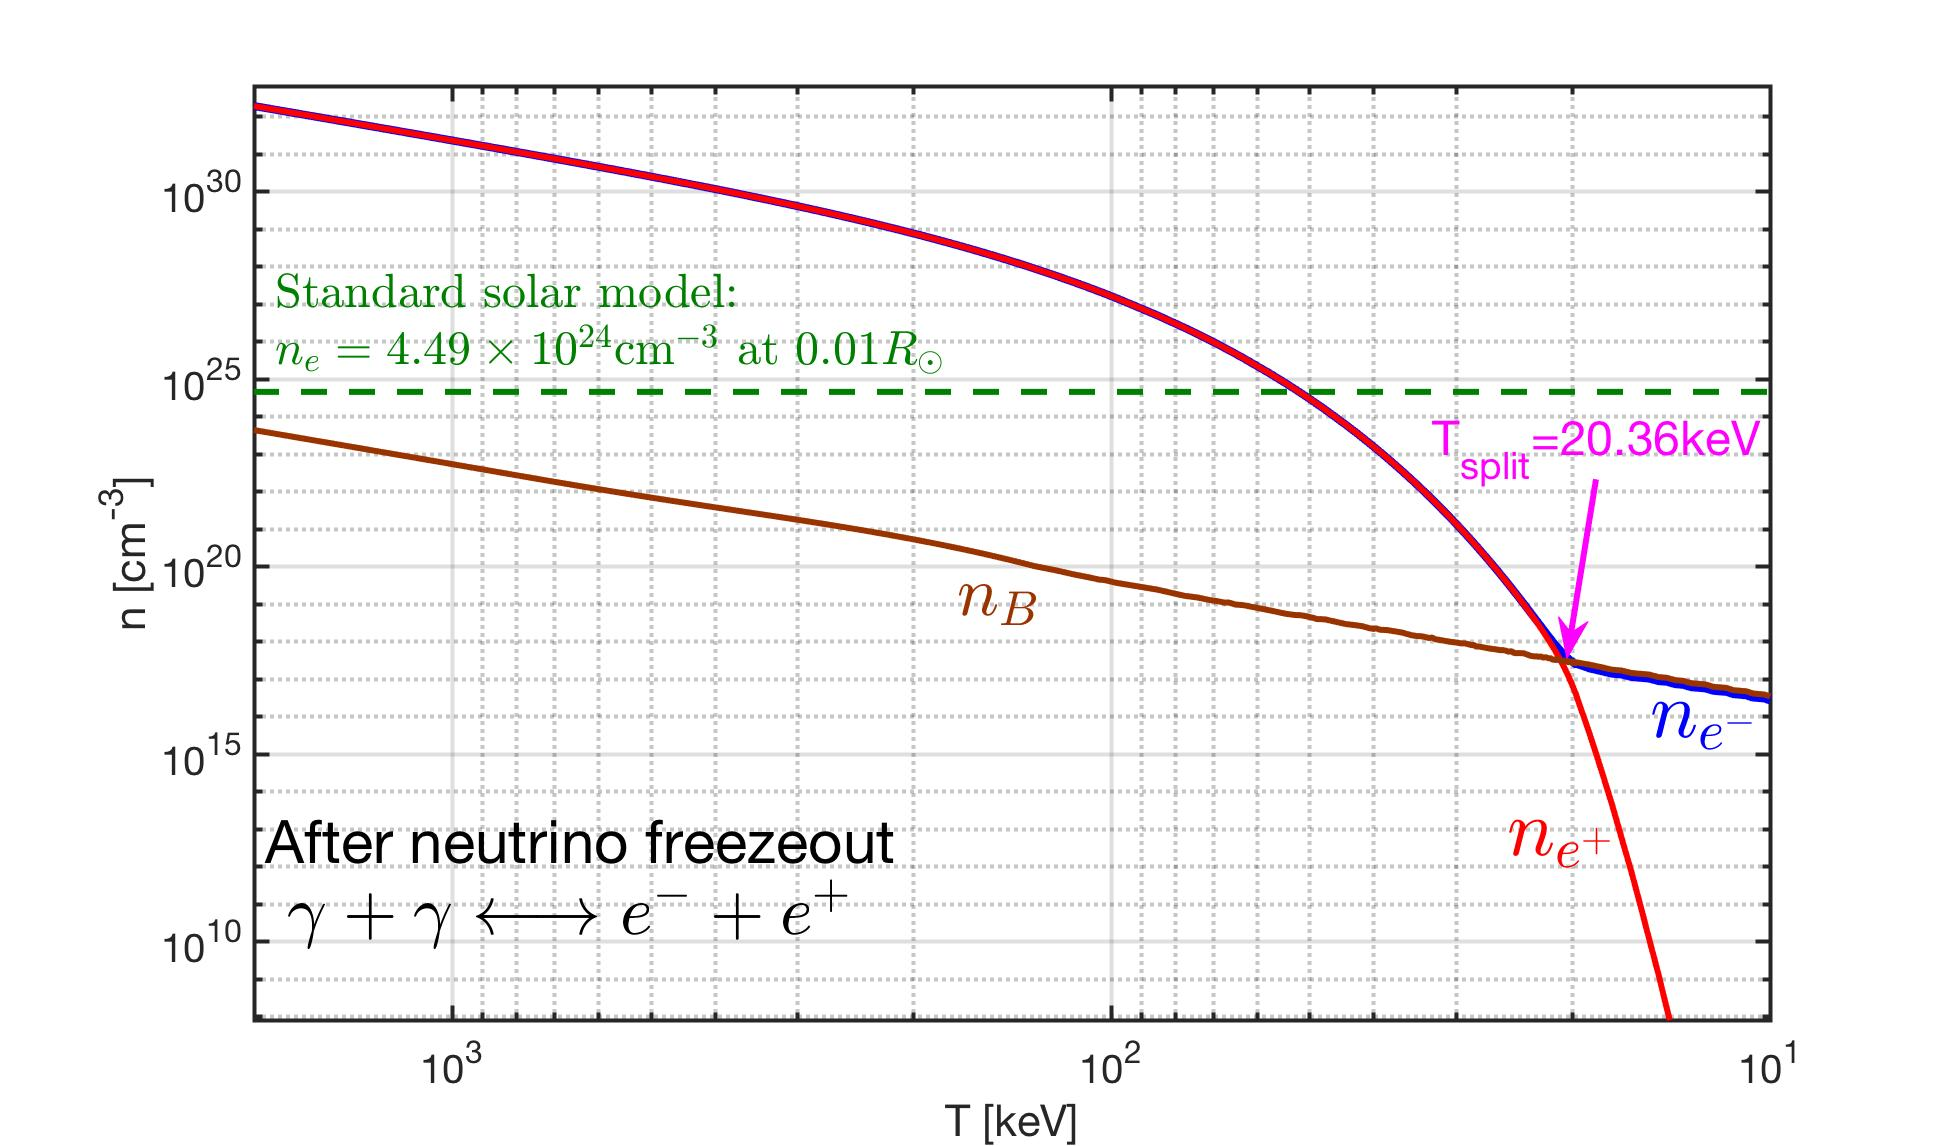
\includegraphics[width=\linewidth]{./plots/NewDensity_cm3.jpg}
  \caption{The electron(positron) number density as a function of temperature in the range $2\,\mathrm{MeV}>T>10\,\mathrm{keV}$. The blue solid line is the electron density, the red solid line is the positron density, and the brown solid line is the baryon density. For comparison, we also show the green dotted line as the solar electron density within the stellar core. This reveals we have an electron-positron rich plasma in early universe until $T_{\mathrm{split}} = 20.36\ \mathrm{keV}$, for $T<T_{\mathrm{split}}$ the positron density quickly vanishes because of annihilation leaving only a residual electron density as required by charge conservation.}
  \label{Density_fig} 
\end{figure}
%%%%%%%%%%%%%%%%%%%%%%%%%%%%%%%%%%%%%%%

\section{Standard Cosmology}\label{sec:Cosmo}
%%%%%%%%%%%%%%%%%%%%%%%%%%%%%%%
\noindent Here we provide background on the standard  cosmological (FLRW-Universe) model that is used in the computation of the compositive of the universe over time. We use the spacetime metric
\beqn\label{metric}
ds^2=c^2dt^2-a^2(t)\left[ \frac{dr^2}{1-kr^2}+r^2(d\theta^2+\sin^2(\theta)d\phi^2)\right]
%g_{00}=1, \quad g_{rr}=-\frac{a^2}{1-kr^2}, \quad g_{\theta\theta}=-a^2r^2, \quad g_{\phi\phi}=-a^2 r^2\sin^2\theta
\eeqn
characterized  by the scale parameter $a(t)$  of a spatially homogeneous  Universe. The geometric parameter $k$ identifies the geometry of the spacial hypersurfaces defined by comoving observers. Space is a flat-sheet for the observationally preferred value $k=0$ \cite{Planck}. In this case it can be more convenient to write the metric in rectangular coordinates
\beqn\label{metric2}
ds^2=c^2dt^2-a^2(t)\left[ dx^2+dy^2+dz^2\right].
\eeqn
We will work in units where $\hbar=1,c=1$.

The global Universe dynamics can be characterized by two  quantities: the Hubble parameter  $H$, a strongly time dependent quantity on cosmological time scales,  and the deceleration parameter $q$:
\beqn\label{dynamic}
\frac{\dot a }{a}\equiv H(t) ,\quad \frac{\ddot a}{a}=-qH^2,\quad 
q\equiv -\frac{a\ddot a}{\dot a^2},\quad \dot H=-H^2(1+q). 
\eeqn

The Einstein equations are:
\beqn\label{Einstine}
G^{\mu\nu}=R^{\mu\nu}-\left(\frac R 2 +\Lambda\right) g^{\mu\nu}=8\pi G_N T^{\mu\nu},  
\quad R= g_{\mu\nu}R^{\mu\nu}.
\eeqn
Symmetry considerations imply that the stress energy tensor is determined by an energy density and an isotropic pressure
\begin{align}
 T^\mu_\nu =\mathrm{diag}(\rho, -P, -P, -P).
\end{align}
It is common to absorb the Einstein cosmological constant $\Lambda$ into the energy and pressure
\beqn\label{EpsLam}
\rho_\Lambda=\frac{\Lambda}{8\pi G_N}, \qquad P_\Lambda=-\frac{\Lambda}{8\pi G_N}
\eeqn
and we implicitly consider this done from now on.

Two dynamically independent equations arise using the metric \req{metric} in \req{Einstine}:
\beqn\label{hubble}
\frac{8\pi G_N}{3} \rho =  \frac{\dot a^2+k}{a^2}
=H^2\left( 1+\frac { k }{\dot a^2}\right),
\qquad
\frac{4\pi G_N}{3} (\rho+3P)  =-\frac{\ddot a}{a}=qH^2.
\eeqn
We can eliminate the strength of the interaction, $G_N$,  solving both these equations for ${8\pi G_N}/{3}$, and equating the result to find a relatively simple constraint for the deceleration parameter:
\beqn\label{qparam}
q=\frac 1 2 \left(1+3\frac{P}{\rho}\right)\left(1+\frac{k}{\dot a^2}\right).
\eeqn
For a spatially flat Universe, $k=0$, note that in a  matter-dominated era where $P/\rho<<1$ we have $q\simeq 1/2$; for a radiative Universe where $3P=\rho$ we find $q= 1 $; and  in a dark energy Universe in which $P=-\rho$  we find $q=-1$.  Spatial flatness is equivalent to the assertion that the energy density of the Universe equals the critical density
\begin{equation}\label{crit_density}
\rho=\rho_{\text{crit}}\equiv \frac{3H^2}{8\pi G_N}.
\end{equation}

 The CMB power spectrum is sensitive to the  deceleration parameter  and the presence of spatial curvature modifies $q$. The Planck results~\cite{Planck} constrain  the effective curvature energy density fraction,
\begin{equation}
\Omega_K\equiv1-\rho/\rho_{\text{crit}},
\end{equation}
to
\begin{equation}
|\Omega_K|<0.005.
\end{equation}
This indicates a nearly flat Universe. We will work here within an exactly spatially flat cosmological model, $k=0$.  


As must be the case for any solution of Einstein's equations,   \req{hubble} implies that the energy momentum tensor of matter is divergence free:
\beqn\label{divTmn}
T^{\mu\nu};_\nu =0 \Rightarrow -\frac{\dot\rho}{\rho+P}=3\frac{\dot a}{a}=3H.
\eeqn
A dynamical evolution equation for $\rho(t)$ arises once we combine \req{divTmn} with \req{hubble},  eliminating $H$.   Given an equation of state $P(\rho)$, solutions of this equation describes the dynamical evolution of matter in the Universe. In practice, we evolve the system in both directions in time.  On one side, we start in the present era with the energy density fractions fit by Planck data, 
\cite{Planck}
\begin{equation}\label{Planck_params}
H_0=67.74\text{km/s/Mpc},\hspace{2mm} \Omega_b=0.05,\hspace{2mm} \Omega_c=0.26, \hspace{2mm}\Omega_\Lambda=0.69,
\end{equation}
 and integrate backward in time.  On the other hand, we start in the QGP era with an equation of state determined by an ideal gas of SM particles, combined with a perturbative QCD equation of state for quarks and gluons \cite{Borsanyi:2013bia}, and integrate forward in time.

%%%%%%%%%%%%%%%%%%%%%%%%%%%%%%%%%%%%%%%
\section{QGP Epoch}\label{sec:QGP}

%%%%%%%%%%%%%%%%%%%%%%%%%%%%%%%%%%%%%%%
\begin{figure}[h]
  %\begin{center}
  \centering
  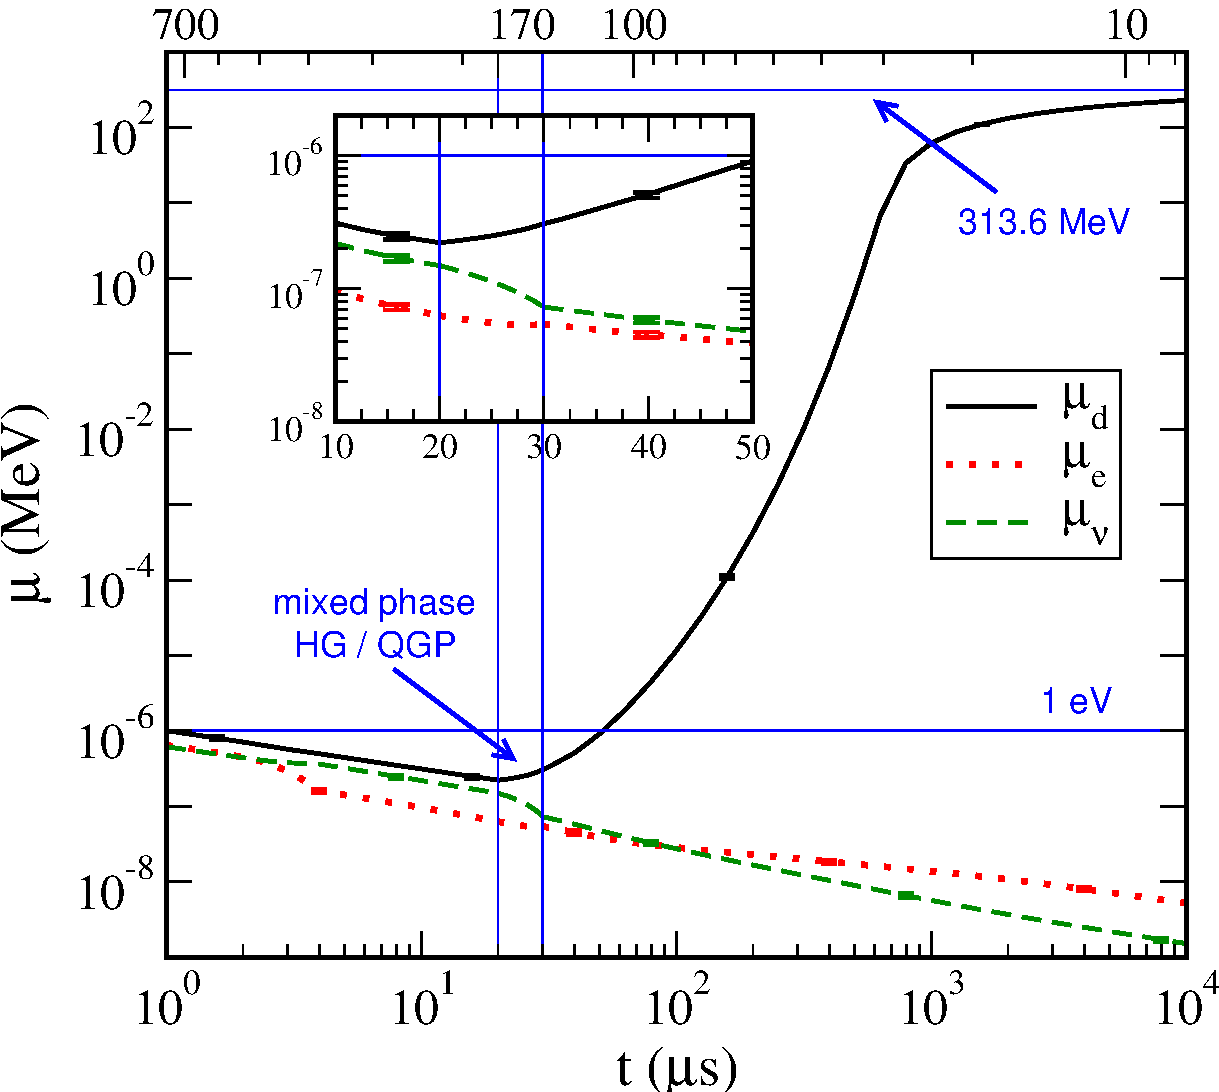
\includegraphics[width=\linewidth]{./extra/muCombo.pdf}
  \caption{TBD.}
  \label{QGPchem} 
\end{figure}
\begin{figure}[h]
  %\begin{center}
  \centering
  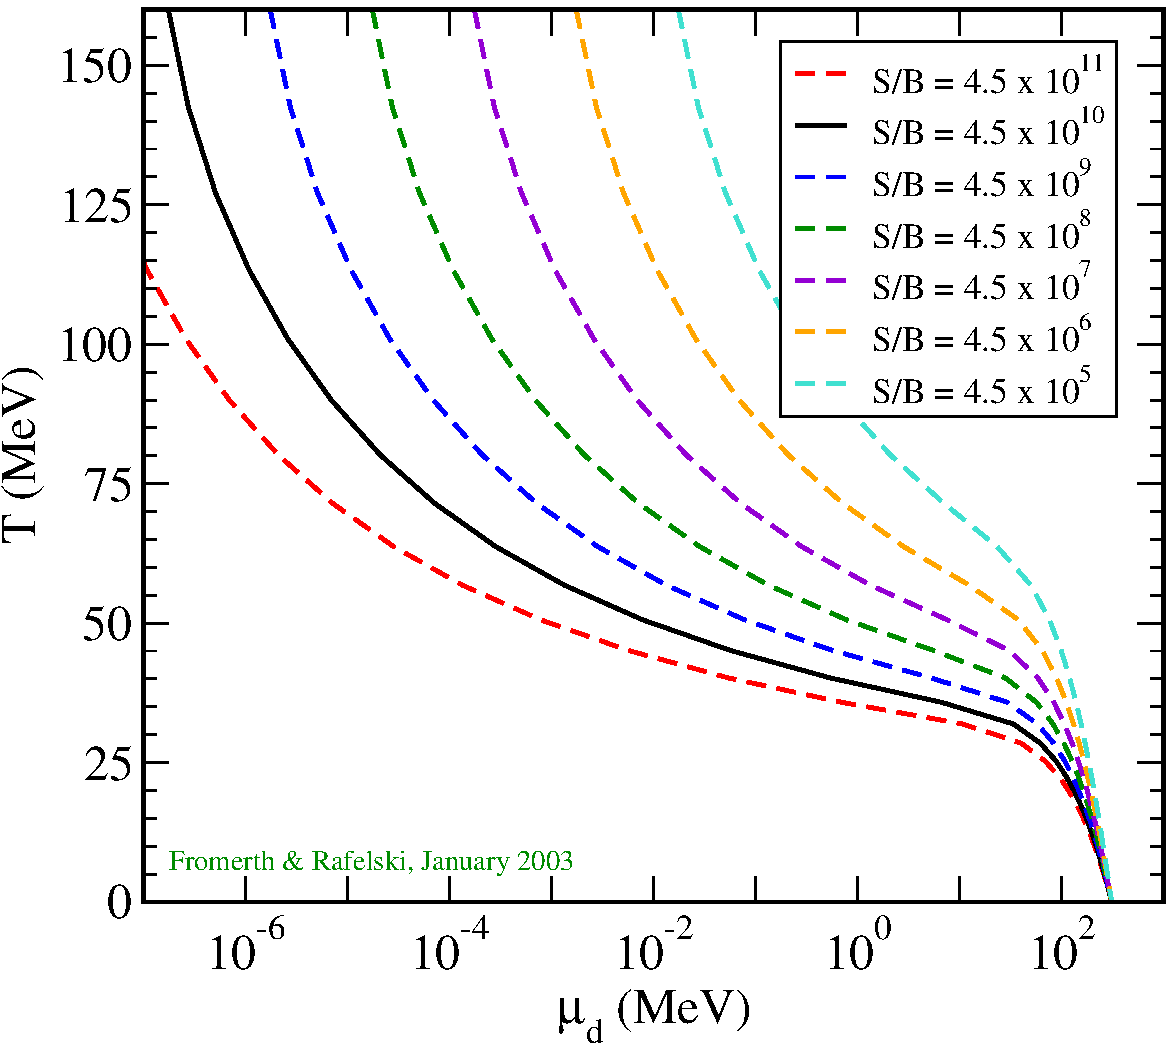
\includegraphics[width=\linewidth]{./extra/Tmud1.pdf}
  \caption{TBD.}
  \label{QGPchem} 
\end{figure}
%%%%%%%%%%%%%%%%%%%%%%%%%%%%%%%%%%%%%%%

%%%%%%%%%%%%%%%%%%%%%%%%%%%%%%%%%%%%%%%
\section{Hadronic Epoch}\label{sec:Hadrons}
The hadron era proceeds with the disappearance of muons, pions, and heavier hadrons.  This constitutes a reheating period, with energy and entropy from these particles being transferred to the remaining $e^\pm$, photon, neutrino plasma.   The black circle near $T=115\MeV$ denotes our change from $2+1$-flavor lattice QCD data for the hadron energy density, taken from Borsanyi et al.~\cite{Borsanyi:2013bia}, to an ideal gas model at lower temperature.  We note that the hadron ideal gas energy density matches the lattice results to less than a percent at $115\MeV$.
\subsection{Cosmological Strangeness Abundance}\label{subsec:Strangeness}
{\color{blue}Briefly review our strangeness paper \cite{Yang:2021bko} here and investigate the strange particle composition of the expanding early Universe in the hadron epoch $150>T>10$ MeV}

\subsection{Pion Abundance in the Early Universe}\label{subsec:Pions}
{\color{blue}Briefly review Inga's paper \cite{Kuznetsova:2008jt} here and show that the $\pi$ is always in chemical equilibrium via the reaction $\gamma\gamma\to\pi^0$}

%In general $\pi^0$ in the cosmic plasma is produced predominantly  in the thermal two photon fusion:
%\begin{equation}
%\gamma+\gamma \rightarrow \pi^0. \label{pi0gg}
%\end{equation}
%Much less probable is the production of $\pi_0$ in the reaction:
%\begin{equation}
%e^-+e^+ \rightarrow \pi^0. \label{pi0ee}
%\end{equation}
%These formation processes are the inverse of the decay process of $\pi_0$.The smallness of the electro-formation of $\pi_0$ is characterized by the small  branching ratio in $\pi_0$ decay $B=\Gamma_{ee}/\Gamma_{\gamma\gamma}=6.2\pm 0.5 10^{-8}$.
%Other decay processes involve more than two particles. $\pi^0$ can also be formed by charged pions in charge exchange reactions. However, in electron positron plasma in the domain of $T$ of interest we find that at first the neutral pions will be produced. These
%in turn produce charged pions.


%%%%%%%%%%%%%%%%%%%%%%%%%%%%%%%%%%%%%%%
\section{Electron-Positron-Neutrino Epoch}\label{sec:ElectronPositronNeutrino}
\subsection{The muon abundance in the early univese}\label{sec:Muons}
Muon abundance is an important quantity required for the understanding of several fundamental questions regarding properties of the primordial Universe. Our interest in strangeness flavor freeze-out in the early Universe \cite{Yang:2021bko} requires the understanding of the abundance of muons in the early Universe. The specific question needing an answer is at which temperature muons remain in abundance (chemical) equilibrium established predominantly by electromagnetic and weak interaction processes, allowing detailed-balance back-reactions to influence strangeness abundance.

In the the cosmic plasma muons can be produced by the interaction processes 
\begin{align} 
&\gamma+\gamma\longrightarrow\mu^++\mu^-,\qquad & e^++e^-\longrightarrow \mu^++\mu^-\;,\\
&\pi^-\longrightarrow\mu^-+\bar{\nu}_\mu,\qquad & \pi^+\longrightarrow\mu^++\nu_\mu\;.
\end{align}
The back reaction for all above processes is in detailed balance, provided all particles shown on the right hand side (RHS) exist in chemical abundance equilibrium in the Universe. We recall the vacuum life time of pions $\tau_\pi=2.6033\times10^{-8}$ sec. 

However, all produced muons can decay 
\begin{equation}
\mu^-\rightarrow\nu_\mu+e^-+\bar{\nu}_e,\qquad \mu^+\rightarrow\bar{\nu}_\mu+e^++\nu_e\,
\end{equation} 
with the vacuum life time $\tau_{\mu}=2.197 \times 10^{-6}\mathrm{sec}$. In the paper \cite{Rafelski:2021aey} we evaluate the production and decay rates of muons in the cosmic plasma as a function of temperature. This allows to determine when exactly the muon abundance disappears. In Fig(\ref{muon_fig}) we show the invariant thermal reaction rates per volume and time for the relvance muon reactions. By comparing the production and decay rates we obtain the temperature at which muons disappear from the universe is $T_\mathrm{dis} = 4.20$ MeV.

%%%%%%%%%%%%%%%%%%%%%%%%%%%%%%%%%%%%%%%
\begin{figure}[h]
%\begin{center}
\centering
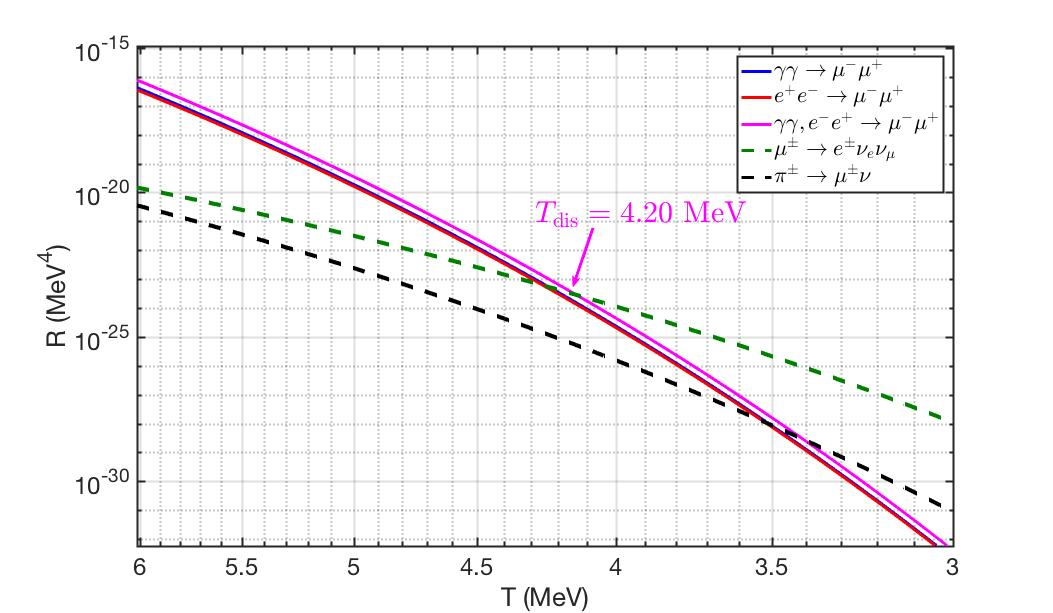
\includegraphics[width=\linewidth]{MuonRate_New3.jpg}
\caption{The thermal reaction rate per volume for different reactions as a function of temperature adapted from paper \cite{Rafelski:2021aey}. It shows that dominant reactions for $\mu^\pm$ production are ${\gamma+\gamma\to\mu^++\mu^-}$ and $e^++e^-\to\mu^++\mu^-$, and the total production rate cross the decay rate of $\mu^\pm$ at temperature $T_\mathrm{dis}\approx 4.20$ MeV.}
\label{muon_fig} 
\end{figure}
%%%%%%%%%%%%%%%%%%%%%%%%%%%%%%%%%%%%%%%

As the temperature decreases in the expanding Universe, the initially dominant production rates become smaller faster and cross the decay rates. Muon abundance disappears as soon as any decay rate is faster than the fastest production rate. Considering the slow speed of the Universe expansion the muon disappearance is sudden, the muon abundance thus disappears as soon as a decay rate crosses the dominant production rate. Specifically after the Universe cools below the temperature $T_\mathrm{dis} = 4.20$ MeV, the dominant reaction is the muon decay.

The density ratio at $T=T_\mathrm{dis}$ is $n_{\mu^\pm}/n_\mathrm{B}\approx0.91$. This means that the muon abundance may still be able to influence baryon evolution because their number density is comparable to the baryon density. This offers a new and tantalizing model building opportunity for  baryon-antibaryon separation in the primordial Universe, strangelet formation, and perhaps other exotic primordial structure formation mechanisms.

%%%%%%%%%%%%%%%%%%%%%%%%%%%%%%%%%%%%%%%
\subsection{Neutrino freezeout in early universe}\label{sec:Freezeout}
\noindent The relic neutrino background is believed to be a  well preserved probe of a Universe only a second old. The properties of the neutrino background are influenced by the details of the freeze-out or decoupling process at a temperature $T=\mathcal{O}(1\,MeV)$. In general The freeze-out process, whereby a particle species stops interacting and decouples from the photon background, involves several steps that lead to the final form of the free-streaming momentum distribution. We outline the freezeout properties, including what distinguishes it from the equilibrium distributions as follow\cite{Birrell:2012gg}:
\begin{itemize}
  \item
Chemical freeze-out of a particle species occurs at the temperature, 
$T_{ch}$, when particle number changing processes slow down and the particle abundance can no longer be maintained at an equilibrium level. Prior to the  chemical freeze-out temperature,  number changing processes are significant and keep the particle in chemical (and thermal) equilibrium, implying that the distribution function has the Fermi-Dirac form, obtained by maximizing entropy at fixed energy
\begin{equation}\label{equilibrium}
f_{c}(t,E)=\frac{1}{\exp(E/T)+1}, \text{ for } T(t)> T_{ch}.
\end{equation}

\item
Kinetic freeze-out occurs at the temperature, $T_f$, when momentum exchanging interactions no longer occur rapidly enough to maintain an equilibrium momentum distribution. When $T_f<T(t)<T_{ch}$, number changing process  no longer occur rapidly enough to keep the distribution in chemical equilibrium but there is still sufficient momentum exchange to keep the distribution in thermal equilibrium.  The distribution function is therefore obtained by maximizing entropy, with a fixed energy, particle number, and antiparticle number separately,  implying that the distribution function has the form
\begin{equation}\label{kinetic_equilib}
f_k(t,E)=\frac{1}{\Upsilon^{-1}\exp(E/T)+1}, \text{ for }T_f< T(t)< T_{ch}.
\end{equation}
The fugacity
\begin{equation}
\Upsilon(t)\equiv e^{\sigma(t)}
\end{equation}
 controls the occupancy of phase space and is necessary once $T(t)<T_{ch}$ in order to conserve particle number. See \cite{Birrell:2012gg} for a detailed discussion of its significance.
 
\item
For $T(t)<T_f$ there are no longer any significant interactions that couple the particle species of interest and so they begin to free-stream through the Universe, i.e. travel on geodesics without scattering.  The Einstein Vlasov equation can be solved, see \cite{Choquet-Bruhat:2009xil}, to yield the free-streaming momentum distribution
\begin{equation}\label{free_stream_dist}
f(t,E)=\frac{1}{\Upsilon^{-1}e^{\sqrt{p^2/T^2+m^2 /T_f^2}}+ 1}
\end{equation}
where the free-streaming effective temperature
\begin{equation}\label{T_freestream_dist}
T(t)=\frac{T_fa(t_k)}{a(t)}
\end{equation}
is obtained by redshifting the temperature at kinetic freeze-out. The corresponding free-streaming energy density, pressure, and number densities are given by
\begin{align}
\rho&=\frac{d}{2\pi^2}\!\int_0^\infty\!\!\!\frac{\left(m^2+p^2\right)^{1/2}p^2dp }{\Upsilon^{-1}e^{\sqrt{p^2/T^2+m^2/T_f^2}}+ 1},\label{freestream_rho}\\[0.2cm]
P&=\frac{d}{6\pi^2}\!\int_0^\infty\!\!\!\frac{\left(m^2+p^2\right)^{-1/2}p^4dp }{\Upsilon^{-1} e^{\sqrt{p^2/T^2+m^2/T_f^2}}+ 1},\label{freestream_P}\\[0.2cm]
n&=\frac{d}{2\pi^2}\!\int_0^\infty\!\!\!\frac{p^2dp }{\Upsilon^{-1}e^{\sqrt{p^2/T^2+m^2/T_f^2}}+ 1},
\label{num_density}
\end{align}
where $d$ is the degeneracy of the particle species. These differ from the corresponding expressions for an equilibrium distribution in Minkowski space by the replacement $m\rightarrow m T(t)/T_f$  {\em only} in the exponential. 
\end{itemize}
The separation of the freeze-out process into these three regimes is of course only an approximation.  In principle there is a smooth transition between them.  However, it is a very useful approximation in cosmology.  See \cite{Mangano:2005cc,Birrell:2014gea} for methods capable of resolving these smooth transitions.


%%%%%%%%%%%%%%%%%%%%%%%%%%%%%%%%%%%%%%%
\begin{figure}[h]
\centerline{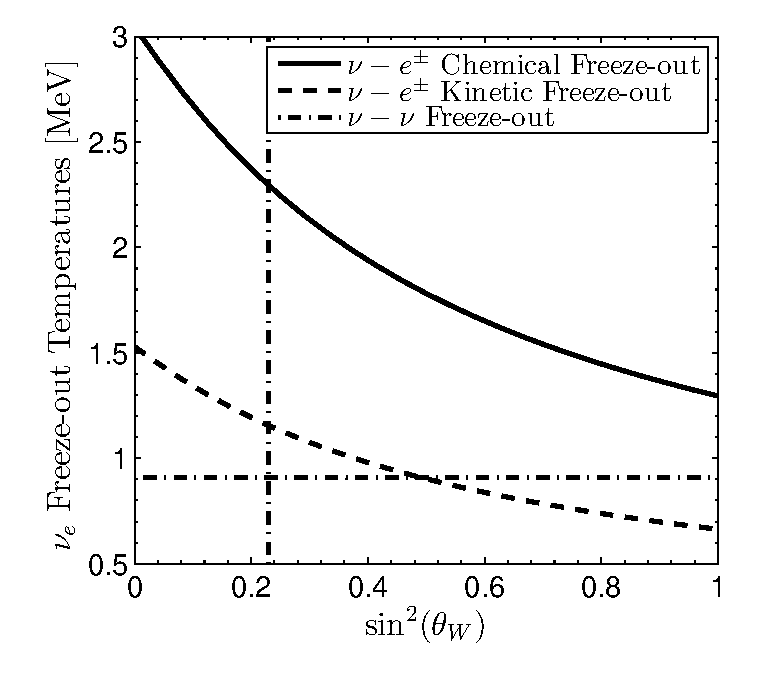
\includegraphics[width=0.47\columnwidth]{nu_e_freezeout.eps}
\hspace{1mm}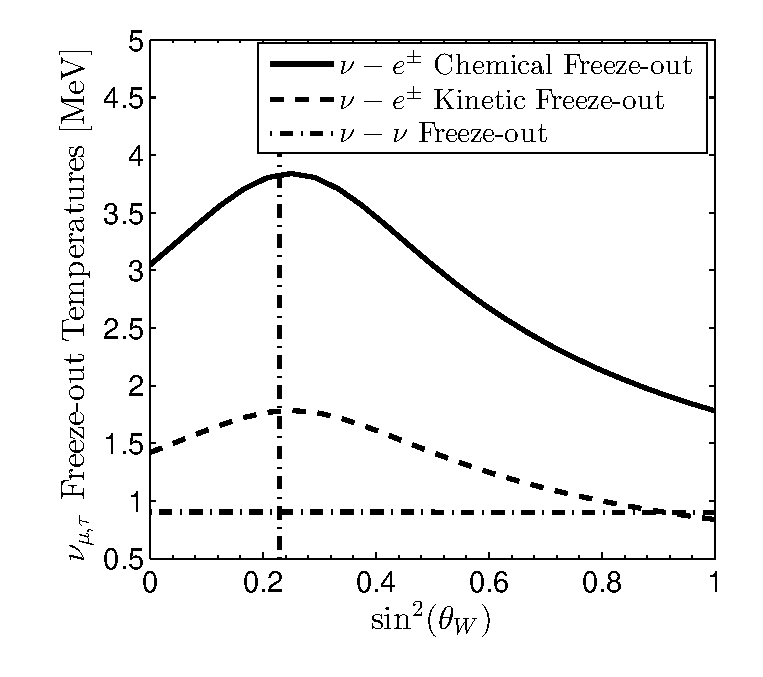
\includegraphics[width=0.47\columnwidth]{nu_mu_freezeout.eps}}
\centerline{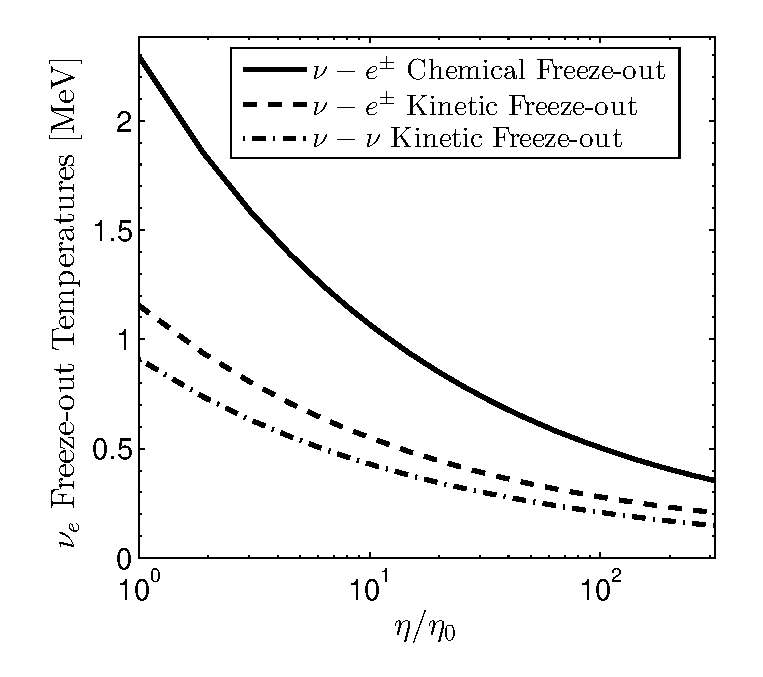
\includegraphics[width=0.47\columnwidth]{nu_e_freezeout_GF.eps}
\hspace{1mm}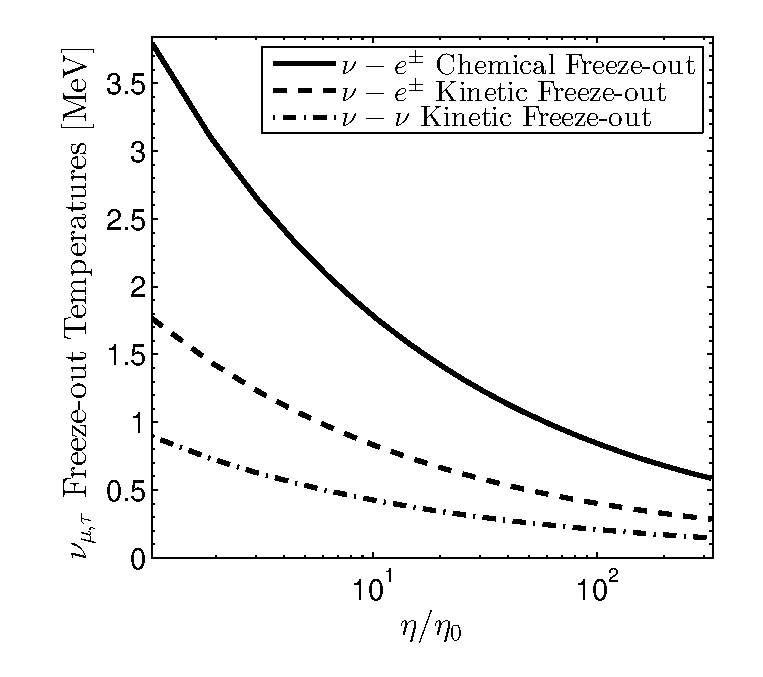
\includegraphics[width=0.47\columnwidth]{nu_mu_freezeout_GF.eps}}
\caption{Freeze-out temperatures for electron neutrinos (left) and $\mu$, $\tau$ neutrinos (right) for the three types of processes adapted from paper \cite{Birrell:2014uka}. Top panels as functions of $\sin^2\theta_W$ for $\eta=\eta_0$, vertical line is $\sin^2\theta_W=0.23$; bottom panels  as a function  of relative change in interaction strength $\eta/\eta_0$ obtained  for $\sin^2\theta_W=0.23$ .}\label{fig:freezeoutT}%\label{fig:Weinberg_freezeout}\label{fig:GF_freezeout}
 \end{figure}
%%%%%%%%%%%%%%%%%%%%%%%%%%%%%%%%%%%%%%%

 To estimate the freezeout temperature we need to solve the Boltzmann equation with different types of collision terms. In paper\cite{Birrell:2014uka} we detail a new method for analytically simplifying the collision integrals and show that the neutrino freezeout temperature which is in turn controlled by the standard model (SM) of particle physics  parameters. The freezeout temperature depends only on the magnitude of the Weinberg angle in the form $\sin^2\theta_W$ , and a dimensionless relative interaction strength parameter $\eta$,
\begin{align}
\eta\equiv M_p m_e^3 G_F^2, \qquad M_p^2\equiv \frac{1}{8\pi G_N}, \end{align}
a combination of  the electron mass $m_e$, Newton constant $G_N$, and the Fermi constant $G_F$. The dimensionless interaction strength parameter $\eta$ with the vacuum present-day value is given by
\begin{align}
\eta_0\equiv \left.M_p m_e^3 G_F^2\right|_0  = 0.04421 .
\end{align}
The magnitude of  $\sin^2\theta_W$ is not fixed within the SM and  could be subject to variation as a function of time or temperature. In Fig.(\ref{fig:freezeoutT}) we show the dependence of neutrino freezeout temperatures for $\nu_e$ and $\nu_{\mu,\tau}$ on SM model parameters  $\sin^2\theta_W$ and $\eta$ in detail.

 The impact of SM parameter values on neutrino freeze-out and the discussion of the implications and connections of this work to other areas of physics, namely Big Bang nucleosynthesis and dark radiation can be found in detail in paper\cite{Birrell:2014uka}


 After neutrinos freezeout, the neutrino comoving entropy is independently conserved. However, the presence of electron-positron rich plasma until $T=20$keV provides the reaction $\gamma\gamma\to e^-e^+\to\nu\bar{\nu}$ to occur even after netruinos decouple from the cosmic plasma. This suggest the small amount of $e^\pm$ entropy can still transfer to neutrinos until temperature $T=20$ keV and can free streaming distribution and the effective number of neutrino. 
%%%%%%%%%%%%%%%%%%%%%%%%%%%%%%%%%%%%%%%
\section{Electron-Positron Epoch}\label{sec:ElectronPositron}
The electron-positron epoch of the early universe was home to several significant events which have greatly shaped our contemporary universe including neutrino decoupling, Big Bang Nucleosynthesis (BBN), the annihilation of most electrons and positrons partially re-ionizing the universe, as well as setting the stage for the eventual recombination period which would generate the cosmic microwave background (CMB). Therefore, correctly describing the dynamics of this $e^{\pm}$ plasma is of interest when considering modern cosmic mysteries such as the origin of extra-galactic magnetic fields (EGMF). While most approaches tackle magnetized plasmas from the perspective of magneto-hydrodynamics (MHD), a primarily classical or semi-classical approach, our perspective is to demonstrate that fundamental quantum statistical analysis can lead to further insights on the behavior of magnetized plasmas.

The properties of the electron-positron $e^{\pm}$ plasma in the early universe has not received appropriate attention in an era of precision BBN studies~\cite{Pitrou:2018cgg}. The presence of $e^{\pm}$ pairs before and during BBN has been acknowledged by Wang, Bertulani and Balantekin~\cite{Wang:2010px} over a decade ago. This however was before necessary tools were developed to explore the connection between electron and neutrino plasmas~\cite{Mangano:2005cc,Birrell:2012gg,Birrell:2014uka}. 

In \rf{Density_fig} we show that the dense $e^{\pm}$ plasma in early universe under the hypothesis charge neutrality and entropy conservation as a function of temperature $2\,\mathrm{MeV}>T>10\,\mathrm{keV}$ \cite{Chris:2023abc}. The plasma is electron-positron rich, i.e, $n_{\pm}\gg n_B$ in the early universe until leptonic annihilation at $T_{\mathrm{split}} = 20.36\ \mathrm{keV}$. For $T<T_{\mathrm{split}}$ the positron density $n_{e^+}$ decreases dramatically because of annihilation and the residual electron density becomes equal to the proton density in accordance with charge neutrality in the universe as a whole.
\begin{figure}[htbp]
  \centering  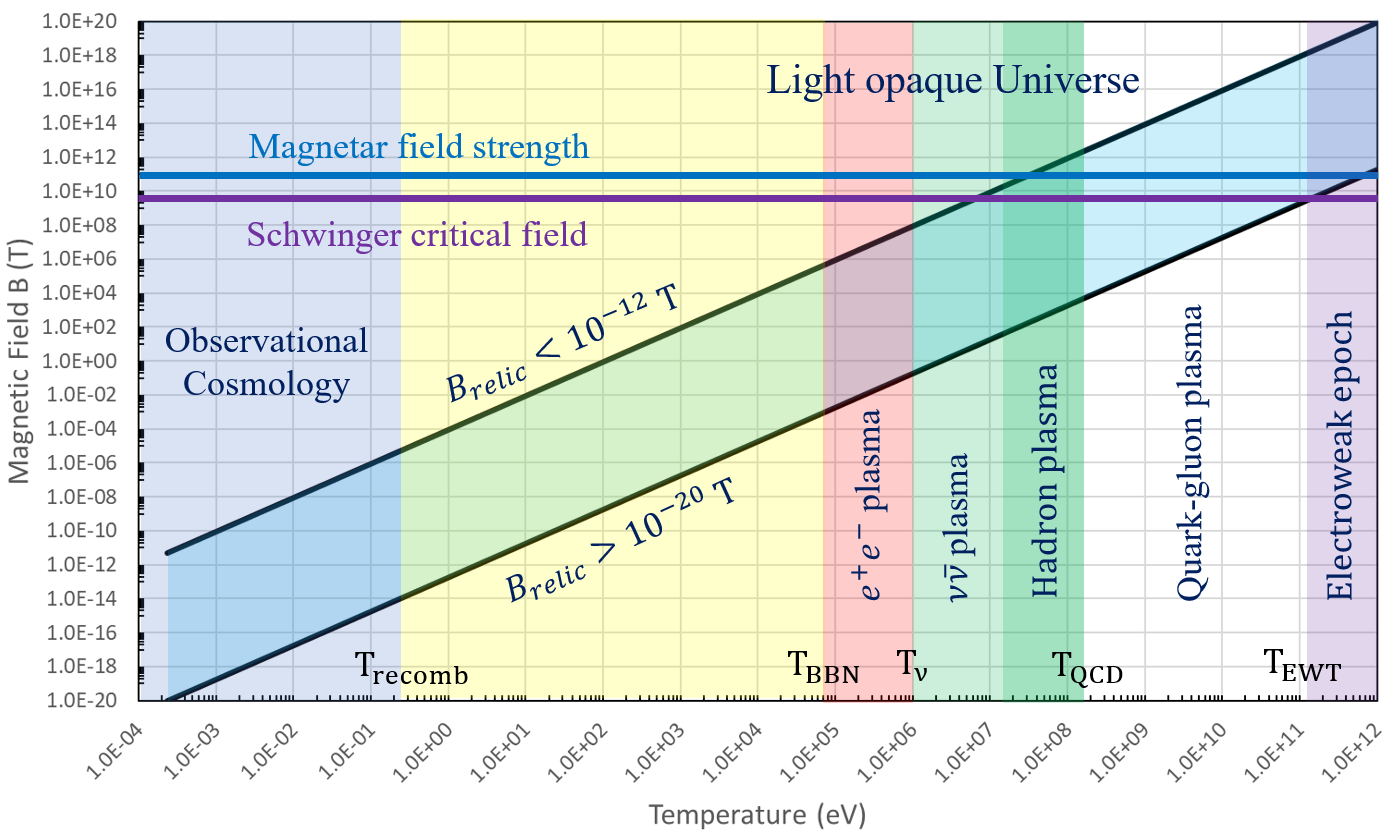
\includegraphics[trim=110 50 120 40,clip,width=\textwidth]{./plots/relic_plot.PDF}
  \label{relic_plot}
  \caption{Qualitative value of the primordial magnetic field over the evolutionary lifespan of the universe. As magnetic flux is conserved over co-moving surfaces, the primordial relic field is expected to dilute as $B\propto1/a(t)^{2}$ meaning the contemporary small bounded values of $5\times10^{-12}\ \mathrm{T}>B_{relic}>10^{-20}\ \mathrm{T}$ may have once represented large magnetic fields in the early universe. This is relic magnetic field would then be generated by the last phase of significant magnetization in the early universe. This figure is meant to be illustrative and it is unlikely the magnetization of the universe would proceed unhindered and unaltered into the ultra-dense plasma phases of the early universe. The values of the Schwinger critical field and the upper bound of surface magnetar field strength are included for scale.}
\end{figure}

We can now connect back to the consideration of cosmic magnetic fields as they might have risen in the environment of early universe plasmas noting that such primordial magnetic fields would be lensed through each of the various plasmas that existed when the universe was far hotter and denser. Of particular interest to us is the electron-positron plasma which existed in the early universe especially at temperatures $T>35\ \mathrm{keV}$ which was the last matter(antimatter) plasma in the universe where the energy its density exceeded that of the proton/neutron baryon energy density. This dense plasma environment is where BBN occurred and where similar plasmas can still be found within exotic stars such as magnetars. The contemporary relic magnetic fields may then be an artifact of this final time of universe-scale magnetization in a manner similar to how the CMB is a relic of the time of charge recombination.

The universe is filled with magnetic fields at various scales and strengths both within galaxies and in deep extra-galactic space far and away from matter sources. Extra-galactic magnetic fields are not well constrained today, but are required by observation to be non-zero with a magnitude between $10^{-12}\ \mathrm{T}>B_{EGMF}>10^{-20}\ \mathrm{T}$ over Mpc coherent length scales. The upper bound is constrained from the characteristics of the CMB while the lower bound is constrained by non-observation of ultra-energetic photons from blazars. There are generally considered two possible origins for extra-galactic magnetic fields: (a) matter-induced dynamo processes involving Amperian currents and (b) primordial (or relic) seed magnetic fields whose origins may go as far back as the Big Bang itself. It is currently unknown which origin accounts for extra-galactic magnetic fields today or if it some combination of the two models. Even if magnetic fields in the universe today are primarily driven via amplification through Amperian matter currents, such models still require primordial seed fields at some point to act as catalyst.
\subsection{Electron-Positron Density Compared to Baryons}\label{subsec:ElectronPositronDensity}
\begin{itemize}
  \item {\xred Explain why matter dynamics is dominated by leptonic matter/antimatter rather than the baryons in this epoch.}
\end{itemize}
Considering the energy density between nonrealtivistc $e^\pm$ and baryon, it can be written as
\begin{align}\label{Eq_ratio}
\chi\equiv\frac{\rho_e+\rho_{\bar e}}{\rho_p+\rho_n}=\frac{m_e(n_e+n_{\bar e})}{m_pn_p+m_n n_n}=\frac{m_e(n_e+n_{\bar e})}{n_B(m_pX_p+m_nX_n)}=\left(\frac{n_e+n_{\bar e}}{n_B}\right)\,\left(\frac{m_e}{m_pX_p+{m_n X_\alpha}/2}\right)
\end{align}
where we consider all neutrons end up bound in to the $^4H_e$ after BBN  and from particle data group $X_p=n_p/n_B$ and $X_\alpha=n_\alpha/n_B$ and are given by
\begin{align}
X_p=0.878,\qquad X_\alpha=0.245
\end{align}
and masses are given by
\begin{align}
m_e=0.511\,\mathrm{MeV}, \qquad m_p=938.272\,\mathrm{MeV},\qquad m_n=939.565\,\mathrm{MeV}
\end{align}
In Fig.(\ref{ratio_fig}) we plot the energy density ratio Eq.(\ref{Eq_ratio}) as a function of temperature $10\,\mathrm{keV}< T<200\,\mathrm{keV}$. It shows that the energy density of electron and positron is dominated until $T=30.2$ keV, i.e.,  we have $\rho_{e}\gg\rho_B$. After $T=30.2$ keV, we have $\rho_{e}\ll\rho_B$ and ratio becomes constant when is around $T=20$keV because of the positron annihilation and charge neutrality.

%To estimate the energy density ratio for the low temperature limit $T\ll20$ keV, we can consider that all positrons disappear because of the annihilation. Then the energy density ratio becomes:
%\begin{align}
%\chi=\frac{\rho_e+\rho_{\bar e}}{\rho_p+\rho_\alpha}
%&=\left(\frac{n_e}{n_B}\right)\,\left(\frac{m_e}{m_pX_p+m_nX_\alpha/2}\right)=\left(\frac{n_p}{n_B}\right)\,\left(\frac{m_e}{m_pX_p+m_n X_\alpha/2}\right)\\
%&=X_p\,\left(\frac{m_e}{m_pX_p+m_nX_\alpha/2}\right)\approx4.78\times10^{-4}
%\end{align}
%where we use the charge neutrality $n_e=n_p$ to replace the electron density by proton density and we can calculate the ratio by giving the $X_p$ and $X_\alpha$ from observation.

%%%%%%%%%%%%%%%%%%%%%%%%%%%%%%%%%%%%%%%
\begin{figure}[h]
%\begin{center}
\centering
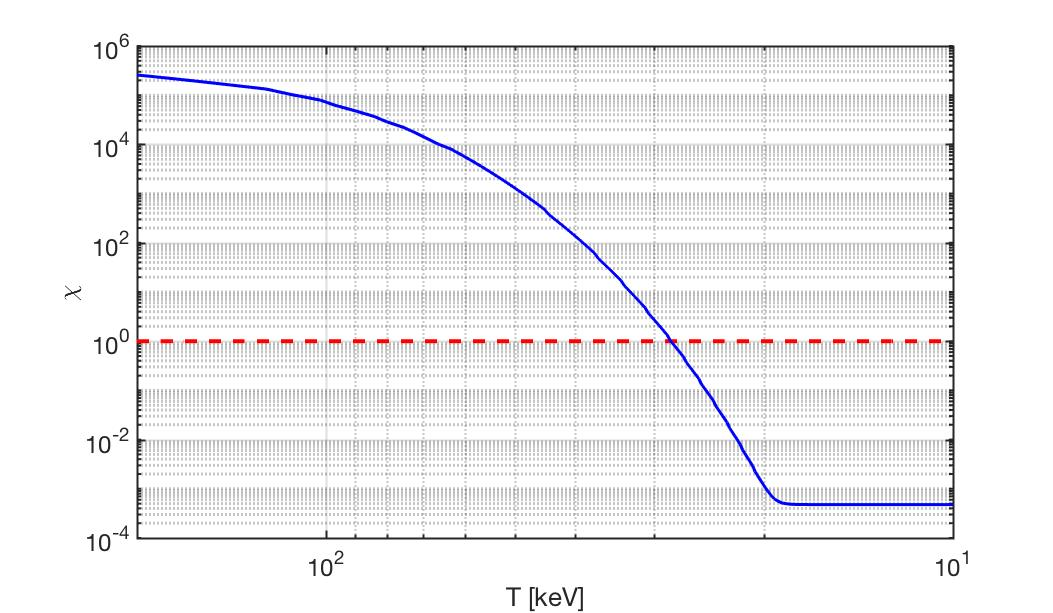
\includegraphics[width=\linewidth]{EnergyDensityRatio002.jpg}
\caption{The energy density ratio Eq.(\ref{Eq_ratio}) as a function of temperature $10\,\mathrm{keV}< T<200\,\mathrm{keV}$. It shows that the energy density of electron and positron is dominated until $T=30.2$ keV, i.e.,  we have $\rho_{e}\gg\rho_B$.}
\label{ratio_fig} 
\end{figure}
%%%%%%%%%%%%%%%%%%%%%%%%%%%%%%%%%%%%%%%
\subsection{Energy Eigenvalues}\label{subsec:energy}
\noindent As a starting point, we consider the energy eigenvalues of charged fermions within a homogeneous magnetic field. Here, we have several choices: We could assume the typical Dirac energy eigenvalues with gyro-magnetic g-factor set to $g=2$. But as electrons, positrons and most plasma species have anomalous magnetic moments (AMM), we require a more complete model. Another option would be to modify the Dirac equation with a Pauli term, often called the Dirac-Pauli (DP) approach, via
\begin{align}
  \label{Pauli} \hat{H}_{\mathrm{AMM}} = -a\frac{e}{2m_{e}}\frac{\sigma_{\mu\nu}F^{\mu\nu}}{2}\,,
\end{align}
where $\sigma_{\mu\nu}$ is the spin tensor proportional to the commutator of the gamma matrices and $F^{\mu\nu}$ is the EM field tensor. For the duration of this work, we will remain in natural units $(\hbar=c=k_{B}=1)$ unless explicitly stated otherwise. The AMM is defined via g-factor as
\begin{align}
  \label{AMM} \frac{g}{2}=1+a\,.
\end{align}
This approach, while straightforward, would complicate the energies making analytic understanding and clarity difficult without a clear benefit. Modifying the Dirac equation with \req{Pauli} yields the following eigen-energies
\begin{align}
  \label{DPEnergy} E_{n}^{s}\vert_{DP}=\sqrt{\left(\sqrt{m_{e}^{2}+2eB\left(n+\frac{1}{2}-s\right)}-\frac{eB}{2m}(g-2)s\right)^{2}+p_{z}^{2}}
\end{align}
This model for the electron-positron plasma of the early universe has been used in work such as Strickland et. al. \cite{Strickland:2012vu}. Our work here is then in part a companion peice which compares and contrasts the DP model of fermions to our preferred model for the AMM via the Klein-Gordon-Pauli (KGP) equation given by
\begin{alignat}{1}
  \label{KGP} \left(\left(i\partial_{\mu}-eA_{\mu}\right)^{2}-m_{e}^{2}-e\frac{g}{2}\frac{\sigma_{\mu\nu}F^{\mu\mu}}{2}\right)\Psi=0\,.
\end{alignat}
We wish to emphasize, that each of the three above models (Dirac, DP, KGP) are distinct and have differing physical consequences and are not interchangeable which we explored in the context of hydrogen-like atoms in \cite{Steinmetz:2018ryf}. Recent work done in \cite{Rafelski:2022bsv} discuss the benefits of KGP over other approaches for $g\neq2$ from a quantum field theory perspective. Exploring the statistical behavior of KGP in a cosmological contenxt can lead to new insights in magnetization which may be distinquished from pure $g=2$ behavior of the Dirac equation or the \emph{ad hoc} modification imposed by the Pauli term in DP. One major improvement of the KGP approach over the more standard DP approach is that the energies take eigenvalues which are mathematically similar to the Dirac energies. Considering the $e^\pm$ plasma in a uniform magnetic field $B$ pointing along the $z$-axis, the energy of $e^\pm$ fermions can be written as
\begin{align}
  \label{KGPEnergy} E_{n}^{s}&=\sqrt{p^2_z+\tilde{m}^2+2eBn},\qquad\tilde{m}^2=m^2_e+eB\left(1-gs\right),\qquad s=\pm\frac{1}{2},\qquad n=0,1,2,3,\dots
\end{align}
where $n$ is the principle quantum number for the Landau levels and $s$ is the spin quantum number. Here we introduce a notion of effective mass $\tilde{m}$ which inherits the spin-specific part of the energy adding them to the mass. This convention is also generalizable to further non-minimal electromagnetic models with more exotic energy contributions such that we write a general replacement as
\begin{align}
  \label{MagMass} m_{e}^{2}\rightarrow\tilde{m}^2(B)\,.
\end{align}
This definition also pulls out the ground state Landau energy separating it from the remainder of the Landau tower of states. One restriction is that the effective mass must remain positive definite in our analysis thus we require
\begin{align}
  \label{MassLimit} \tilde{m}^2(B)=m^2_e+eB\left(1-gs\right)>0\,.
\end{align}
This condition fails under ultra-strong magnetic fields of order
\begin{align}
  \label{MagMassFail} B_{\mathrm{crit}}=\frac{m_{e}^{2}}{ea}=\frac{\mathcal{B}_{S}}{a}\approx3.8\times10^{12}\ \mathrm{T}\,,
\end{align}
where $\mathcal{B}_{S}$ is the Schwinger critical field strength. For electrons, this field strength is well above the window of magnetic field strengths of interest during the late $e^{\pm}$ epoch.

%%%%%%%%%%%%%%%%%%%%%%%%%%%%%%%%%%%%%%%
\subsection{Landau eigen-energies in cosmology}\label{subsec:Landau}
\noindent The standard model of cosmology with a cosmological constant plus cold dark matter ($\Lambda\mathrm{CDM}$) is described by the Friedman-Lemaître-Robertson-Walker (FLRW) metric. The spatially flat (Gaussian curvature $k=0$) FLRW metric with metric signature $(+1,-1,-1,-1)$ in Cartesian coordinates is
\begin{align}
    \label{FLRW} ds^2=dt^2-a^2(t)\left[dx^2+dy^2+dz^2\right]\,.
\end{align}
The scale factor $a(t)$ denotes the change of proper distances in an expanding (or contracting) universe which is both homogeneous and isotropic. The evolutionary expansion of the universe is then traditionally defined in terms of the Hubble parameter $H(t)$ as follows
\begin{align}
  \label{Friedmann} H(t)^{2}\equiv\left(\frac{\dot a}{a}\right)^2=\frac{8\pi G_{N}}{3}\rho_{tot},\quad \frac{\ddot a}{a}=-qH^2,\quad 
q\equiv -\frac{a\ddot a}{\dot a^2},\quad \dot H=-H^2(1+q).
\end{align}
where $G_N$ is the Newtonian constant of gravitation, $\rho_{tot}$ is the total energy density of the universe and $q$ is the cosmic deceleration parameter. \req{Friedmann} is also known as the Friedmann equations. 

There is another natural scale for the magnetic field besides \req{MagMassFail} when considering the consequences of FLRW expansion on the $e^{\pm}$ fluid. As the universe expands, different terms in the energies and thus partition function evolve as a function of the scale factor $a(t)$ which arises in the FLRW metric. We can consider the expansion to be an adiabatic process which results in a smooth shifting of the relevant dynamical quantities. From the conservation of magnetic flux through a co-moving surface, the magnetic field under expansion starting at some initial time $t_{0}$ is given by
\begin{alignat}{1}
    \label{BScale} B(t) = B(t_{0})\frac{a(t_{0})^{2}}{a(t)^{2}}\,.
\end{alignat}
As the universe expands, the temperature also cools as the cosmological redshift reduces the momenta of particles in the universe lowering their contribution to the energy content of the universe. This cosmological redshift is written as
\begin{alignat}{1}
  \label{Redshift} p_{i}(t) = p_{i}(t_{0})\frac{a(t_{0})}{a(t)}\,,\qquad T(t) = T(t_{0})\frac{a(t_{0})}{a(t)}\,.
\end{alignat}
The momenta scale with the same factor as temperature as it is the origin of cosmological redshift. The energy of massive free particles in the universe scales differently based on their momentum (and thus temperature). When hot and relativistic, particle energy scales with inverse scale factors like radiation. However as particles transition to non-relativistic momenta, their energies scale with the inverse square of the scale factor like magnetic flux.
\begin{alignat}{1}
    \label{EScale} E(t) = E(t_{0})\frac{a(t_{0})}{a(t)}\xrightarrow{\mathrm{NR}}\  E(t_{0})\frac{a(t_{0})^{2}}{a(t)^{2}}\,.
\end{alignat}
This occurs because of the functional dependence of energy on momentum in the relativistic versus non-relativistic cases. The argument in the Boltzmann statistical factor is given by
\begin{alignat}{1}
    \label{Boltz} X_{n}^{s}\equiv\frac{E_{n}^{s}}{T}\,.
\end{alignat}
We can explore this relationship for the magnetized system explicitly by writing out \req{Boltz} using the KGP eigen-energies as
\begin{alignat}{1}
    \label{XExplicit} X_{n}^{s} = \sqrt{\frac{m_{e}^{2}}{T^{2}}+\frac{p_{z}^{2}}{T^{2}}+\frac{2eB}{T^{2}}\left(n+\frac{1}{2}-\frac{gs}{2}\right)}\,,
\end{alignat}
where we now introduce the expansion scale factor via \req{BScale} - \req{Redshift}. The Boltzmann factor can then be written as
\begin{alignat}{1}
    \label{XScale} X_{n}^{s}[a(t)] = \sqrt{\frac{m_{e}^{2}}{T^{2}(t_{0})}\frac{a(t)^{2}}{a(t_{0})^{2}}+\frac{p_{z}^{2}(t_{0})}{T^{2}(t_{0})}+\frac{2eB(t_{0})}{T^{2}(t_{0})}\left(n+\frac{1}{2}-\frac{gs}{2}\right)}\,.
\end{alignat}
This reveals that only the mass contribution is dynamic over cosmological time. For any given eigen-state, the mass term increases driving the state into the non-relativistic limit while the momenta and magnetic contributions are frozen by initial conditions. As a point of comparison, the Boltzmann factor for the DP eigen-energies becomes
\begin{alignat}{1}
    \label{XDP} X_{n}^{s}\vert_{DP} = \sqrt{\left(\sqrt{\frac{m_{e}^{2}}{T^{2}}+\frac{2eB}{T^{2}}\left(n+\frac{1}{2}-s\right)}-\frac{eB}{2mT}(g-2)s\right)^{2}+\frac{p_{z}^{2}}{T^{2}}}\,,
\end{alignat}
which over cosmological time under expansion scales as
\begin{alignat}{1}
    \label{XScaleDP} X_{n}^{s}[a(t)]\vert_{DP} = \sqrt{\left(\sqrt{\frac{m_{e}^{2}}{T^{2}(t_{0})}\frac{a(t)^{2}}{a(t_{0})^{2}}+\frac{2eB(t_{0})}{T^{2}(t_{0})}\left(n+\frac{1}{2}-s\right)}-\frac{eB(t_{0})}{2mT(t_{0})}\frac{a(t_{0})}{a(t)}(g-2)s\right)^{2}+\frac{p_{z}^{2}(t_{0})}{T^{2}(t_{0})}}\,.
\end{alignat}
%We note here one important difference between KGP and DP eigen-energies in the context of cosmology: The anomalous magnetic moment portion of the DP statistics is suppressed by $1/a(t)$ over cosmological time while the AMM contribution is preserved in the KGP model. That the universe's expansion makes a distinction between $g=2$ magnetic moment and AMM for DP fermions appears as a rather artificial and nonphysical trait. While the suppression of AMM may often be small for particles such as electrons, this suppression is non-trivial for particles with large AMM values such as the proton. That cosmological redshift would push DP protons to be described by $g=2$ eign-energies in the non-relativistic limit counts as a malaise for the model and further strengthens our thinking that the KGP model is more appropriate for cosmological studies.

\begin{itemize}
    \item {\xred Keep DP cosmo? Note that in NR limit, the magnetic moment is protected in both descriptions contrary to original thoughts.}
\end{itemize}

Motivated by \req{XScale}, we can introduce a dimensionless cosmic magnetic scale which is frozen in the homogeneous case as
\begin{alignat}{1}
    \label{Bo} b_{0}\equiv\frac{eB}{T^{2}}=\frac{eB\hbar c^{2}}{(k_{B}T)^{2}}\ \mathrm{(S.I)}\,,
\end{alignat}
where we've included the expression explicitly in full SI units. We can estimate the value of $b_{0}$ from the bounds on the extra-galactic magnetic field strength and the temperature of the universe today.  If the origin of deep space extra-galactic magnetic fields are relic fields from the early universe, which today are expected to exist between $5\times10^{-12}\ \mathrm{T}>B_{relic}>10^{-20}\ \mathrm{T}$, then at temperature $T=2.7\ \mathrm{K}$, the value of the cosmic magnetic scale is between
\begin{alignat}{1}
    \label{BoScale} 5.5\times10^{-5}>b_{0}>1.1\times10^{-11}\,.
\end{alignat}
This should remain constant in the universe at-large up to the last epoch the universe was sufficiently magnetized to disturb this value. As the electron-proton plasma which generated the CMB was relatively dilute over its duration, it was unlikely sufficiently magnetized to significantly alter this value over extra-galactic scales. Rather, the best candidate plasma to have been sufficiently magnetized and dense to have set the relic field magnetic scale would have been the electron-positron plasma which existed during the duration of Big Bang Nucleosynthesis (BBN) and beforehand.

Higher order non-minimal magnetic contributions which can be introduced via \req{MagMass} to the eigen-energies like $\approx\mu_{B}^{2}B^{2}/T^{2}$ are even more surpressed over cosmological time which drives the system into minimal electromagnetic coupling with the exception of the anomalous magnetic moment in the KGP case. It is interesting to note that cosmological expansion serves to \lq\lq smooth out\rq\rq\ the characteristics of more complex BSM electrodynmaics erasing them from a statistical perspective in favor of the minimal or minimal-like dynamics. As $b_0$ is a constant of expansion, assuming the electron-proton plasma between the CMB and electron-positron annihilation did not greatly disturbed it, we can calculate the remnant values at the temperature $T=50\ \mathrm{keV}$ with the expression
\begin{align}
  \label{BBNFields} B(T)=\frac{b_{0}}{e}T^{2}\,,
\end{align}
yielding a range of field strengths
\begin{align}
  \label{BBNRange} 2.3\times10^{5}\ \mathrm{T}>B(T=50\ \mathrm{keV})>4.6\times10^{-4}\ \mathrm{T}\,,
\end{align}
during which the electron-positron plasma in the universe had a number density comparable to that of the Solar core with $n_{e}=4.49\times10^{24}\ \mathrm{cm}^{-3}$ at $r=0.01R_{\odot}$.

%%%%%%%%%%%%%%%%%%%%%%%%%%%%%%%%%%%%%%%
\subsection{Electron-positron statistical physics}\label{subsec:Partition}
\noindent We now turn our attention now to the statistical behavior of the $e^{\pm}$ system. We can utilize the general fermion partition function given by
\begin{align}
  \label{PartFunc} \ln\mathcal{Z}=\sum_{\alpha}\ln\left(1+e^{-\beta(E-\eta)}\right)\,,
\end{align}
where $\beta=1/T$, $\alpha$ is the set of all quantum numbers in the system, and $\eta$ is the generalized chemical potential. The magnetized $e^{\pm}$ system should be considered a system of four quantum species: Particles and anti-particles, and spin aligned and anti-aligned. Taken together we consider a system where all electrons and positrons are spin aligned or anti-aligned with the magnetic field $B$ and the partition function of the system is written as
\begin{align}
  \label{PartFuncB}\ln\mathcal{Z}_{tot}=\frac{2eBV}{(2\pi)^2}\sum_{\sigma}^{\pm1}\sum_{s}^{\pm1/2}\sum_{n=0}^\infty\int^\infty_{0}dp_z\left[\ln\left(1+\Upsilon_{\sigma}^{s}(x)e^{-\beta E_{n}^{s}}\right)\right]\,,\\
  \label{Fugacity}\Upsilon_{\sigma}^{s}(x)=\gamma(x)\lambda_{\sigma}^{s}\,,\qquad\lambda_{\sigma}^{s}=e^{\sigma\eta_{e}+s\eta_{s}}\,,
\end{align}
where $\eta_{e}$ is the electron chemical potential and $\eta_s$ is the spin chemical potential for the generalized fugacity $\lambda_{\sigma}^{s}$. The parameter $\gamma(x)$ is a spatial field which controls the distribution inhomogeneity of the fermi gas. Inhomogeneities can arrise from the influence of other forces on the gas such as gravitational forces. Deviations of $\gamma\neq1$ represent configurations of reduced entropy (maximum entropy is the regular distribution itself with $\gamma=1$) without pulling the system off a thermal temperature. This is precisely the kind of behavior that may arise in the $e^{\pm}$ epoch as the dominant photon thermal bath keeps the fermi gas in thermal equilibrium while spatial inequilibria could spontanerously develop. The energy $E_{n}^\pm$ can be written as
\begin{align}
E_{n}^\pm&=\sqrt{p^2_z+\tilde m^2_\pm+2eBn},\qquad\tilde{m}^2_\pm=m^2_e+eB\left(1\mp\frac{g}{2}\right)\,,
\end{align}
where the $\pm$ script refers to spin aligned and anti-aligned eigenvalues. As the temperature domain we're interested is in the $T=50\ \mathrm{keV}$ range, we can take a semi-relativistic approach of the electron-positron plasma by considering the partition function obtained in the Boltzmann approximation $k=1$. In following we considering the case $\eta_s/T\ll1$ for the first approximation and Boltzmann approximation for nonrelativistic electrons and positrons. Using the Euler-Maclaurin formula to replace the sum over Landau levels with an integration yielding
\begin{align}
  \ln\mathcal{Z}_{tot}=\ln\mathcal{Z}_{free}+\ln\mathcal{Z}_B+\ln\mathcal{Z}_R\,,
\end{align}
where we define 
\begin{align}
  \label{FreePart}&\ln\mathcal{Z}_{free}=\frac{T^3V}{2\pi^2}\left[2\cosh{\left(\frac{\eta_{e}}{T}\right)}\right]\sum_{i=\pm}x_i^2K_2\left(x_i\right)\,,\\
  \label{MagPart}&\ln\mathcal{Z}_B=\frac{eBTV}{2\pi^2}\left[2\cosh{\left(\frac{\eta_{e}}{T}\right)}\right]\sum_{i=\pm}\bigg[\frac{x_i}{2}K_1\left(x_i\right)+\frac{k^2b_0}{12}K_0\left(x_i\right)\bigg]\,,\\
  \label{ErrorPart}&\ln\mathcal{Z}_R=\frac{eBTV}{\pi^2}\left[2\cosh{\left(\frac{\eta_{e}}{T}\right)}\right]R.
\end{align}
where $R$ is the error remainder which is defined by integrals over Bernoulli polynomials.
While this would require further derivation to demonstrate explicitly, the benefit of the Euler-Maclaurin approach is if the error contribution remains finite or bound for the magnetized partition function, then a correspondence between the free Fermi partition function (with noticeably modified effective mass $\tilde{m}_{\pm}$) and the magnetized Fermi partition function can be established. The mismatch between the summation and integral in the Euler-Maclaurin formula would then encapsulate the immediate magnetic response and deviation from the free particle phase space. While we label $\ln(\mathcal{Z}_{free})$ in \req{FreePart} as the \lq\lq free\rq\rq\ partition function, this is not strictly true as this contribution to the overall partition function is a function of the effective mass we defined earlier in \req{MagMass}. When determining the magnetization of the quantum Fermi gas, derivatives of the magnetic field $B$ will not fully vanish on this first term which will resulting in an intrinsic magnetization which is distinct from the contribution from the ground state and mismatch between the quantized Landau levels and the continuum of the free momentum. Specifically, this free Fermi contribution represents the magnetization that arises from the spin magnetic energy rather than orbital contributions.

Assuming the error remainder $R$ is small and can be neglected, we can rewrite \req{FreePart} - \req{MagPart} obtaining
\begin{align}
  \label{lnZ}
  \ln\mathcal{Z}_{tot}=\frac{T^3V}{2\pi^2}\left[2\cosh\left(\frac{\eta_{e}}{T}\right)\right]\sum_{i=\pm}\left\{x_i^{2} K_2\left(x_i\right)+\frac{b_0}{2}x_iK_1\left(x_i\right)+\frac{b^2_0}{12}K_0\left(x_i\right)\right\}\,.
\end{align}
\req{lnZ} is our working model for the

\subsection{Charge neutrality and chemical potential}
 In this section we are interested in exploring the chemical potential of dense $e\bar e$ plasma in early universe under the hypothesis charge neutrality and entropy conservation. We focus on the temperature interval at post-BBN temperature range $20<T<50$keV. In this case, the charge neutrality can be written as
\begin{align}
  \label{density_proton}
  \left(n_{e}-n_{\bar{e}}\right)=(n_{p})=\left(\frac{n_{p}}{n_{B}}\right)\,\left(\frac{n_{B}}{s_{\gamma,\nu,e}}\right)\,s_{\gamma,\nu,e}= X_p\left(\frac{n_B}{s_{\gamma,\nu}}\right)\,s_{\gamma,\nu},\qquad X_p=\frac{n_p}{n_B}
\end{align}
where $n_B$ is the number density of baryon, and the entropy density is obtained by considering the contribution of $e^\pm$ in entropy density is negligible compared to the photon and neutrino entropy density at post-BBN temperature $20<T<50$keV because the low density $n_e\ll n_{\gamma,\nu}$. 
\begin{itemize}
  \item Since all neutrons end up bound in to the $^4H_e$ after BBN, then the mass fraction of $^4H_e$ can be estimated as \cite{ParticleDataGroup:2022pth}
\begin{align}
X_\alpha=\frac{2(n_n/n_p)}{1+n_n/n_p}=0.245\pm0.03.
\end{align} 
 Solving the ratio $n_n/n_p$ and substituting into the $X_p$, we obtain
\begin{align}
 X_p=\frac{n_p}{n_B}=\frac{n_p}{n_p+n_n}=\frac{1}{1+n_n/n_p}=0.878\pm0.015
\end{align}

  \item Since the comoving baryon number and entropy are conserved, hence the ratio $s_{\gamma,\nu}/n_B$ is conserved, then the entropy per baryon ratio can be written as
\begin{align}
\left(\frac{s_{\gamma,\nu}}{n_B}\right)=\left(\frac{s_{\gamma,\nu}}{n_B}\right)_{\!\!t_0}\!\!=\left(\frac{n_\gamma}{n_B}\right)_{\!\!t_0}\left(\frac{s_\gamma}{n_\gamma}+\frac{n_\nu}{n_\gamma}\frac{s_\nu}{n_\nu}\right)=\left(\frac{n_\gamma}{n_B}\right)_{\!\!t_0}\left[3.601+\frac{9}{4}\left(\frac{T_\nu}{T_\gamma}\right)^{\!\!3}4.202\right],
\end{align}
where the subscript $t_0$ denotes the present-day value and considers all neutrinos are relativistic particles today. The entropy per particle for a boson is $(s/n)_\mathrm{boson}=3.601$ and for a fermion is $(s/n)_\mathrm{fermion}=4.202$. From particle data group and standard big bang model \cite{ParticleDataGroup:2022pth,Kolb:1990vq}, we have
\begin{align}
&5.8\times10^{-10}<\frac{n_B}{n_\gamma}<6.5\times10^{-10},\quad\frac{T_\nu}{T_\gamma}=\left(\frac{4}{11}\right)^{1/3}.
\end{align}

  \item The entropy density at temperature can be written as \cite{Kolb:1990vq}
\begin{align}
s=\frac{2\pi^2}{45}g_sT_\gamma^3,\qquad g_s=\sum_{i=boson}g_i\left(\frac{T_i}{T_\gamma}\right)^3+\frac{7}{8}\sum_{i=fermion}g_i\left(\frac{T_i}{T_\gamma}\right)^3
\end{align}
where $g_s$ is the effective degree of freedom that contribute to the entropy density.  
\end{itemize}
 
On the other hand, given the partition function in Boltzmann limit \req{lnZ} the net number density of electron can be written as
\begin{align}
\left(n_e-n_{\bar e}\right)&=\frac{T}{V}\frac{\partial}{\partial \eta_{e}}\ln\mathcal{Z}_{tot}=\frac{T^3}{2\pi^2}\left[2\sinh{(\eta_{e}/T)}\right]\sum_{i=\pm}\left[x_i^2K_2(x_i)+\frac{b_0}{2}x_i K_1(x_i)+\frac{b^2_0}{12}K_0(x_i)\right]
\end{align}
Using the charge neutrality Eq.(\ref{density_proton}) and solving the chemical potential, we obtain:
\begin{align}\label{ChemicalPotential}
\sinh{(\eta_{e}/T)}&=\frac{2\pi^2}{2T^3}\,\frac{X_p(n_B/s_{\gamma,\nu})s_{\gamma,\nu}}{\sum_{i=\pm}\left[x_i^2K_2(x_i)+\frac{b_0}{2}x_i K_1(x_i)+\frac{b^2_0}{12}K_0(x_i)\right]}\\
&\longrightarrow\frac{2\pi^2n_p}{2T^3}\,\frac{X_p(n_B/s_{\gamma,\nu})s_{\gamma,\nu}}{2x^2K_2(x)},\qquad x=m_e/T,\qquad \mathrm{for}\,\,b_0=0
\end{align}
It shows that for the case $b_0=0$ the chemical potential agrees with our earlier results \cite{Chris:2023abc}.
In {\rf{chemical_fig}}, we solve the Eq.(\ref{ChemicalPotential}) numerically and plot the  chemical potential as a function of temperature $T$. It shows that the chemical potential is not sensitive to the magnetic field because the small value of $b_0=10^{-5}\sim10^{-11}$ and can be neglected in \req{ChemicalPotential}. 

%%%%%%%%%%%%%%%%%%%%%%%%%%%%%%%%%%%%%%%
\begin{figure}[h]
%\begin{center}
\centering
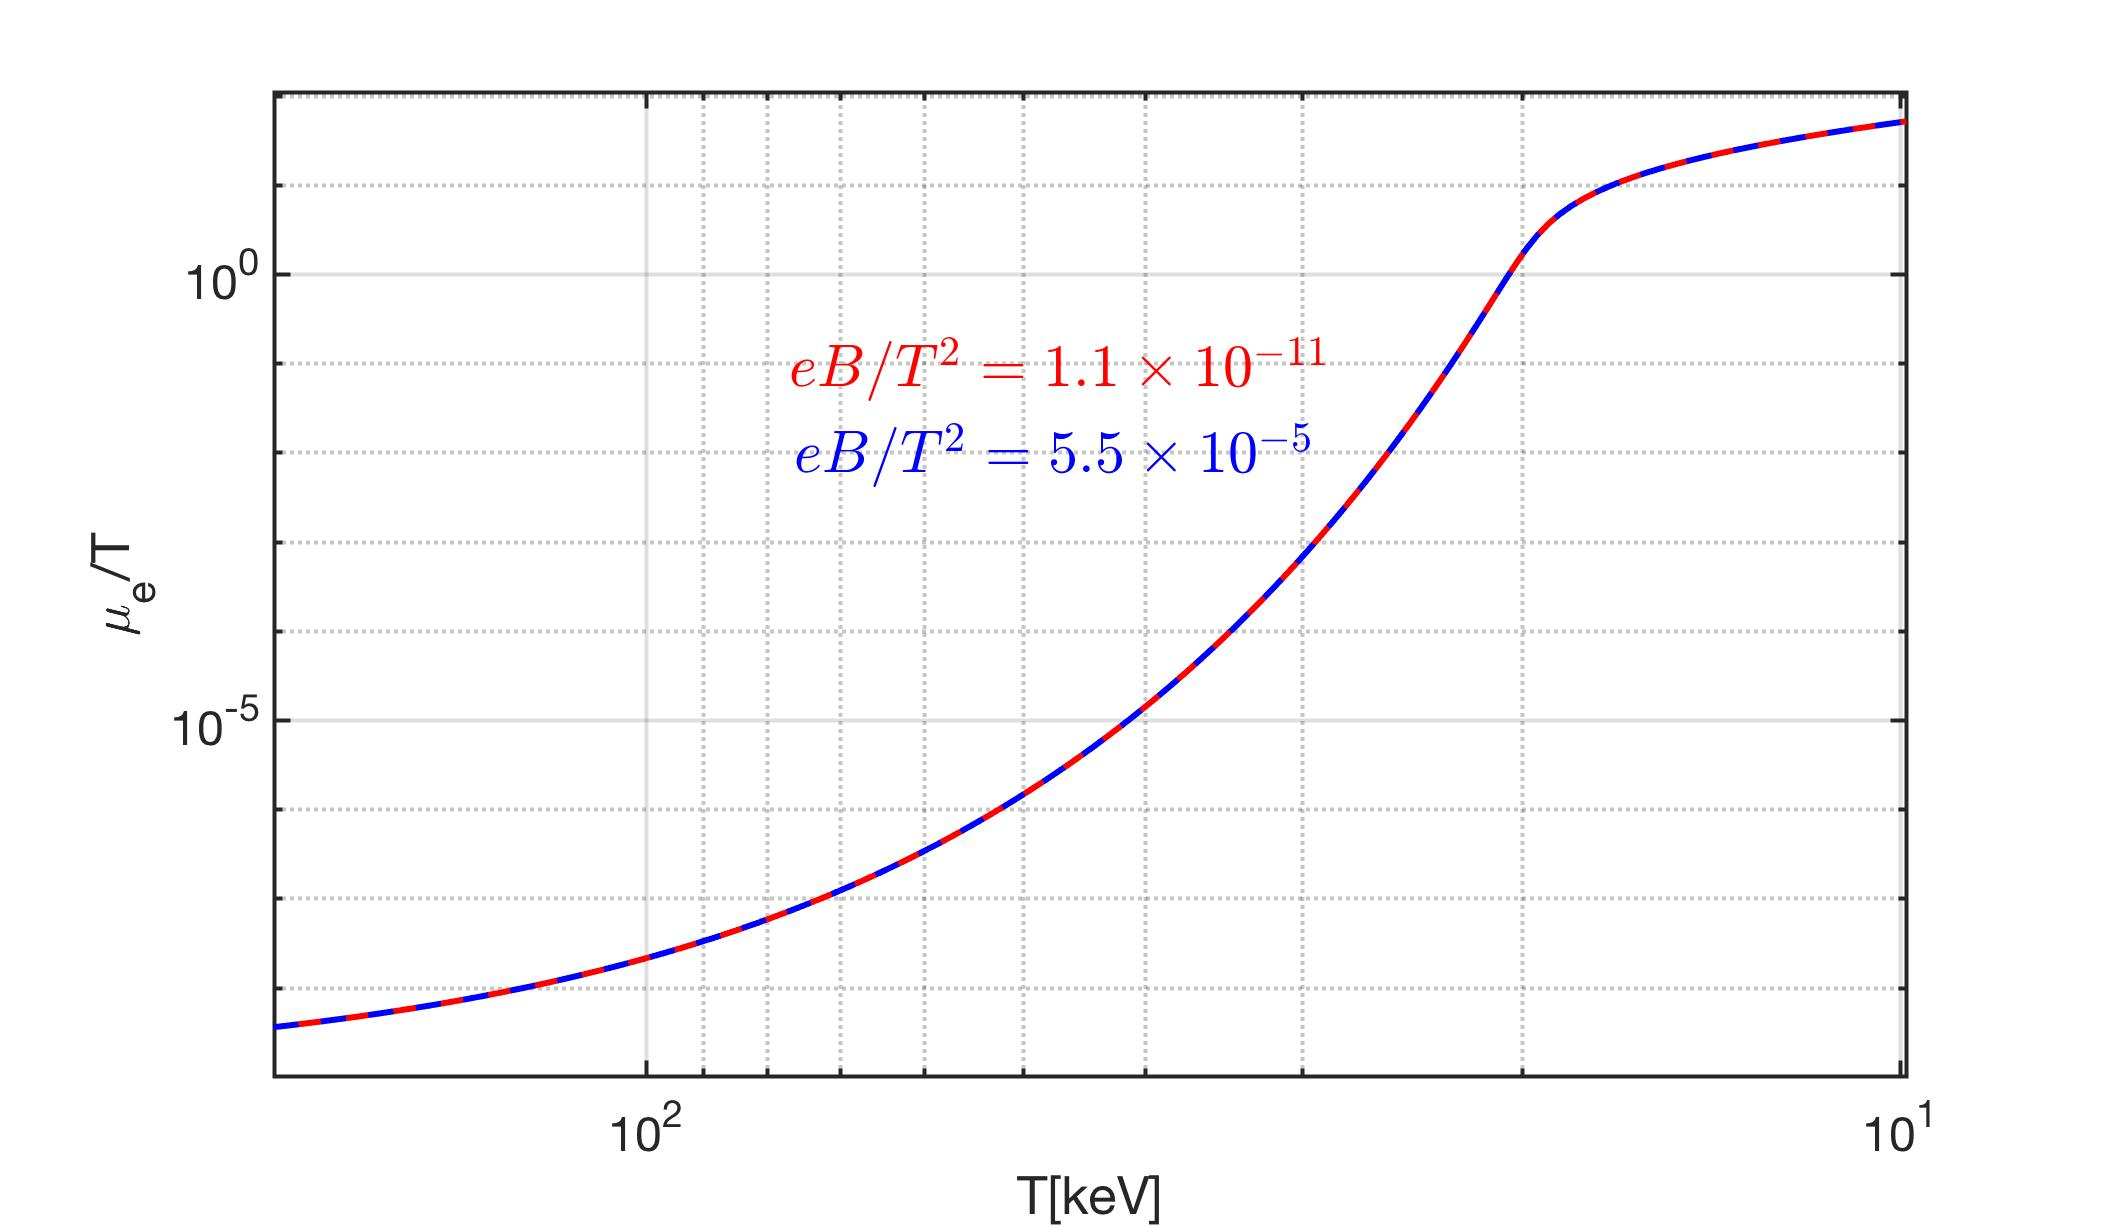
\includegraphics[width=\linewidth]{ChemicalPotentialFinal_200keV.jpg}
\caption{The chemical potential $\eta_{e}/T$ a function of temperature $20<T<60$keV.  It shows that the chemical potential is not sensitive to the magnetic field $b_0$.}
\label{chemical_fig} 
\end{figure}
%%%%%%%%%%%%%%%%%%%%%%%%%%%%%%%%%%%%%%%
In {\rf{chemical_fig}}, we plot the  chemical potential as a function of temperature $T$. It shows that the chemical potential is not sensitive to the magnetic field because the small value of $b_0=10^{-3}\sim10^{-8}$ and can be neglected in \req{ChemicalPotential}. 

%%%%%%%%%%%%%%%%%%%%%%%%%%%%%%%%%%%%%%%
\subsection{Magnetization}\label{subsec:Magnetization}
Given the partition function \req{lnZ} the magnetization can be obtained via the definition
\begin{align}
M=\frac{T}{V}\frac{\partial \ln\mathcal{Z}_{tot}}{\partial B}=\frac{T}{V}\left(\frac{\partial\tilde m_\pm}{\partial B}\right)\frac{\partial \ln\mathcal{Z}_{tot}}{\partial\tilde m_\pm}
\end{align}
then the magnetization can be written as
\begin{align}\label{Magnetization}
\left(\frac{M}{B}\right)=\frac{4\pi\alpha}{2\pi^2b_0}\left[2\cosh\left(\frac{\eta_{e}}{T}\right)\right]\sum_{i=\pm}\left\{\left[\frac{1}{2}-\frac{(1+i g/2)}{2}\left(1+\frac{b^2_0}{12x^2_i}\right)\right]x_i K_1(x_i)+\left[\frac{1}{6}-\frac{(1+ig/2)}{4}\right]b_0K_0(x_i)\right\}.
\end{align}
Substituting the chemical potential \req{ChemicalPotential} into \req{Magnetization} we can solve the magnetization $M/B$ numerically.
Considering the case $g=2$ the magnetization becomes
\begin{align}
\left(\frac{M}{B}\right)=\left(\frac{M}{B}\right)_++\left(\frac{M}{B}\right)
_-
\end{align}
where the functions $(M/B)_\pm$ are defined as 
\begin{itemize}
  \item Case1: $\tilde m_+=\sqrt{m^2_e+2eB}$, and $x_+=\tilde m_+/T$. The magnetization is given by
  \begin{align}\label{Magnetization_001}
 \left(\frac{M}{B}\right)_+&=-\frac{8\pi\alpha}{2\pi^2}\sqrt{1+\sinh^2(\eta_e/T)}\left[\left(\frac{1}{2b_0}+\frac{b_0}{12x_+^2}\right)x_+K_1(x_+)+\frac{1}{3}K_0(x_+)\right]
   \end{align}
Substituting the magnetic field $b_0$ and proton density $n_p/T^3$  we can solve the magnetization and chemical potential numerically. In \rf{Case1_fig}, we plot the  magnetization $M/B$ as a function of temperature $T$. It shows for the case1 the magnetization is not sensitive to the magnetic field, this is because the small value of $b_0=10^{-3}\sim10^{-8}$ and can be neglected in \req{chemical_001} and \req{Magnetization_001}.
\\
  \item Case 2: $\tilde m_-=m_e$ and $x=\tilde m_-/T$,then the magnetization of electron/ positron becomes
\begin{align}\label{Magnetization_002}
\left(\frac{M}{B}\right)_-&=\frac{8\pi\alpha}{2\pi^2}\sqrt{1+\sinh^2(\eta_e/T)}\left(\frac{1}{b_0}x_-K_1(x_-)+\frac{1}{6}K_0(x_-)\right)
\end{align}
Using the magnetic field $b_0$ and proton density $n_p/T^3$ we solve the magnetization  numerically. In \rf{Case2_fig}, we plot the  magnetization $M/B$ as a function of temperature $T$. It shows that the magnetization depends on the magnetic field $b_0$ strongly. This is because for a small magnetic field $b_0$ the dominant term in \req{Magnetization_002} is $xK_1(x)/b_0$. For given $b_0$, the value of magnetization can be larger than the magnetic field, i.e. $M/B>1$  which shows the possibility that magnetic domains can be formed in the early universe.
\end{itemize}
%%%%%%%%%%%%%%%%%%%%%%%%%%%%%%%%%%%%%%%
\begin{figure}[h]
%\begin{center}
\centering
%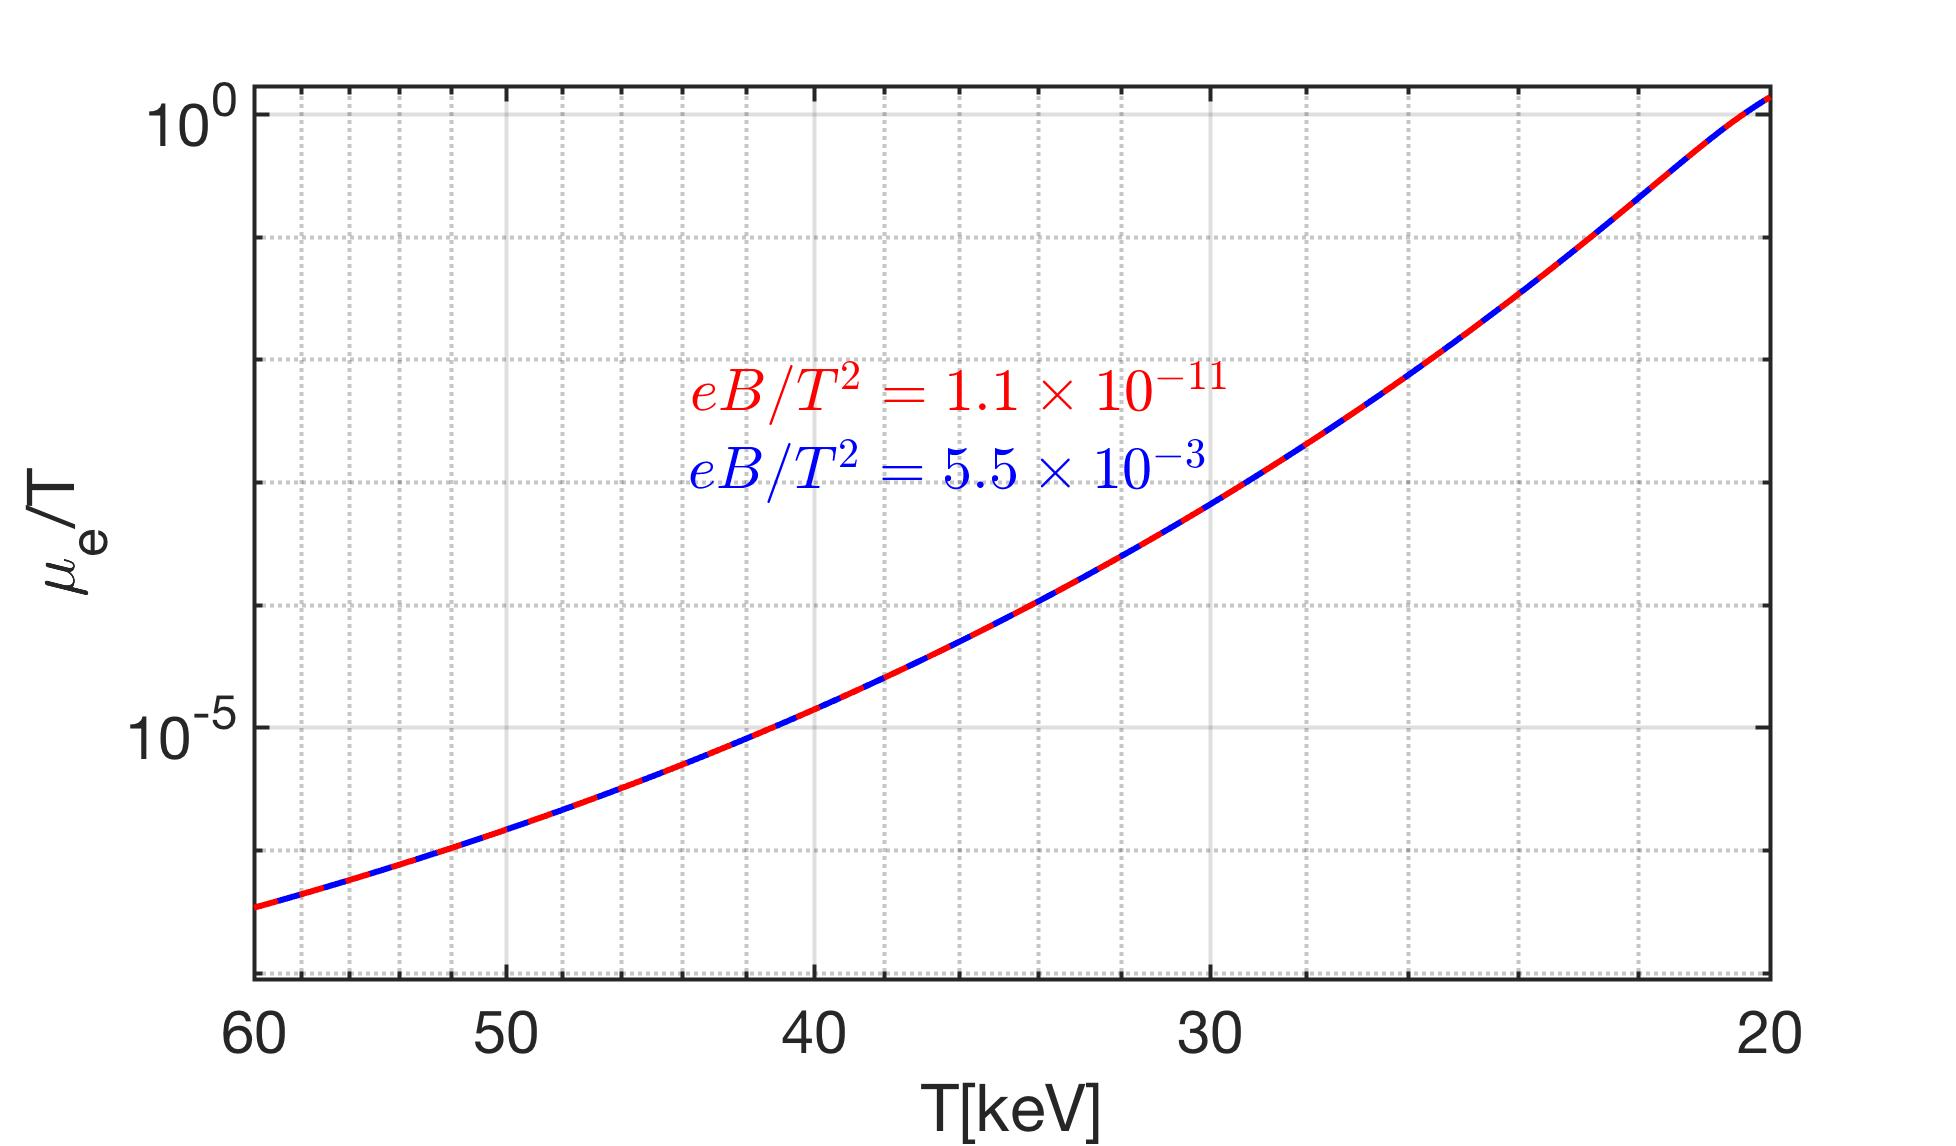
\includegraphics[width=0.75\linewidth]{./plots/ChemicalPotential_case2.jpg}
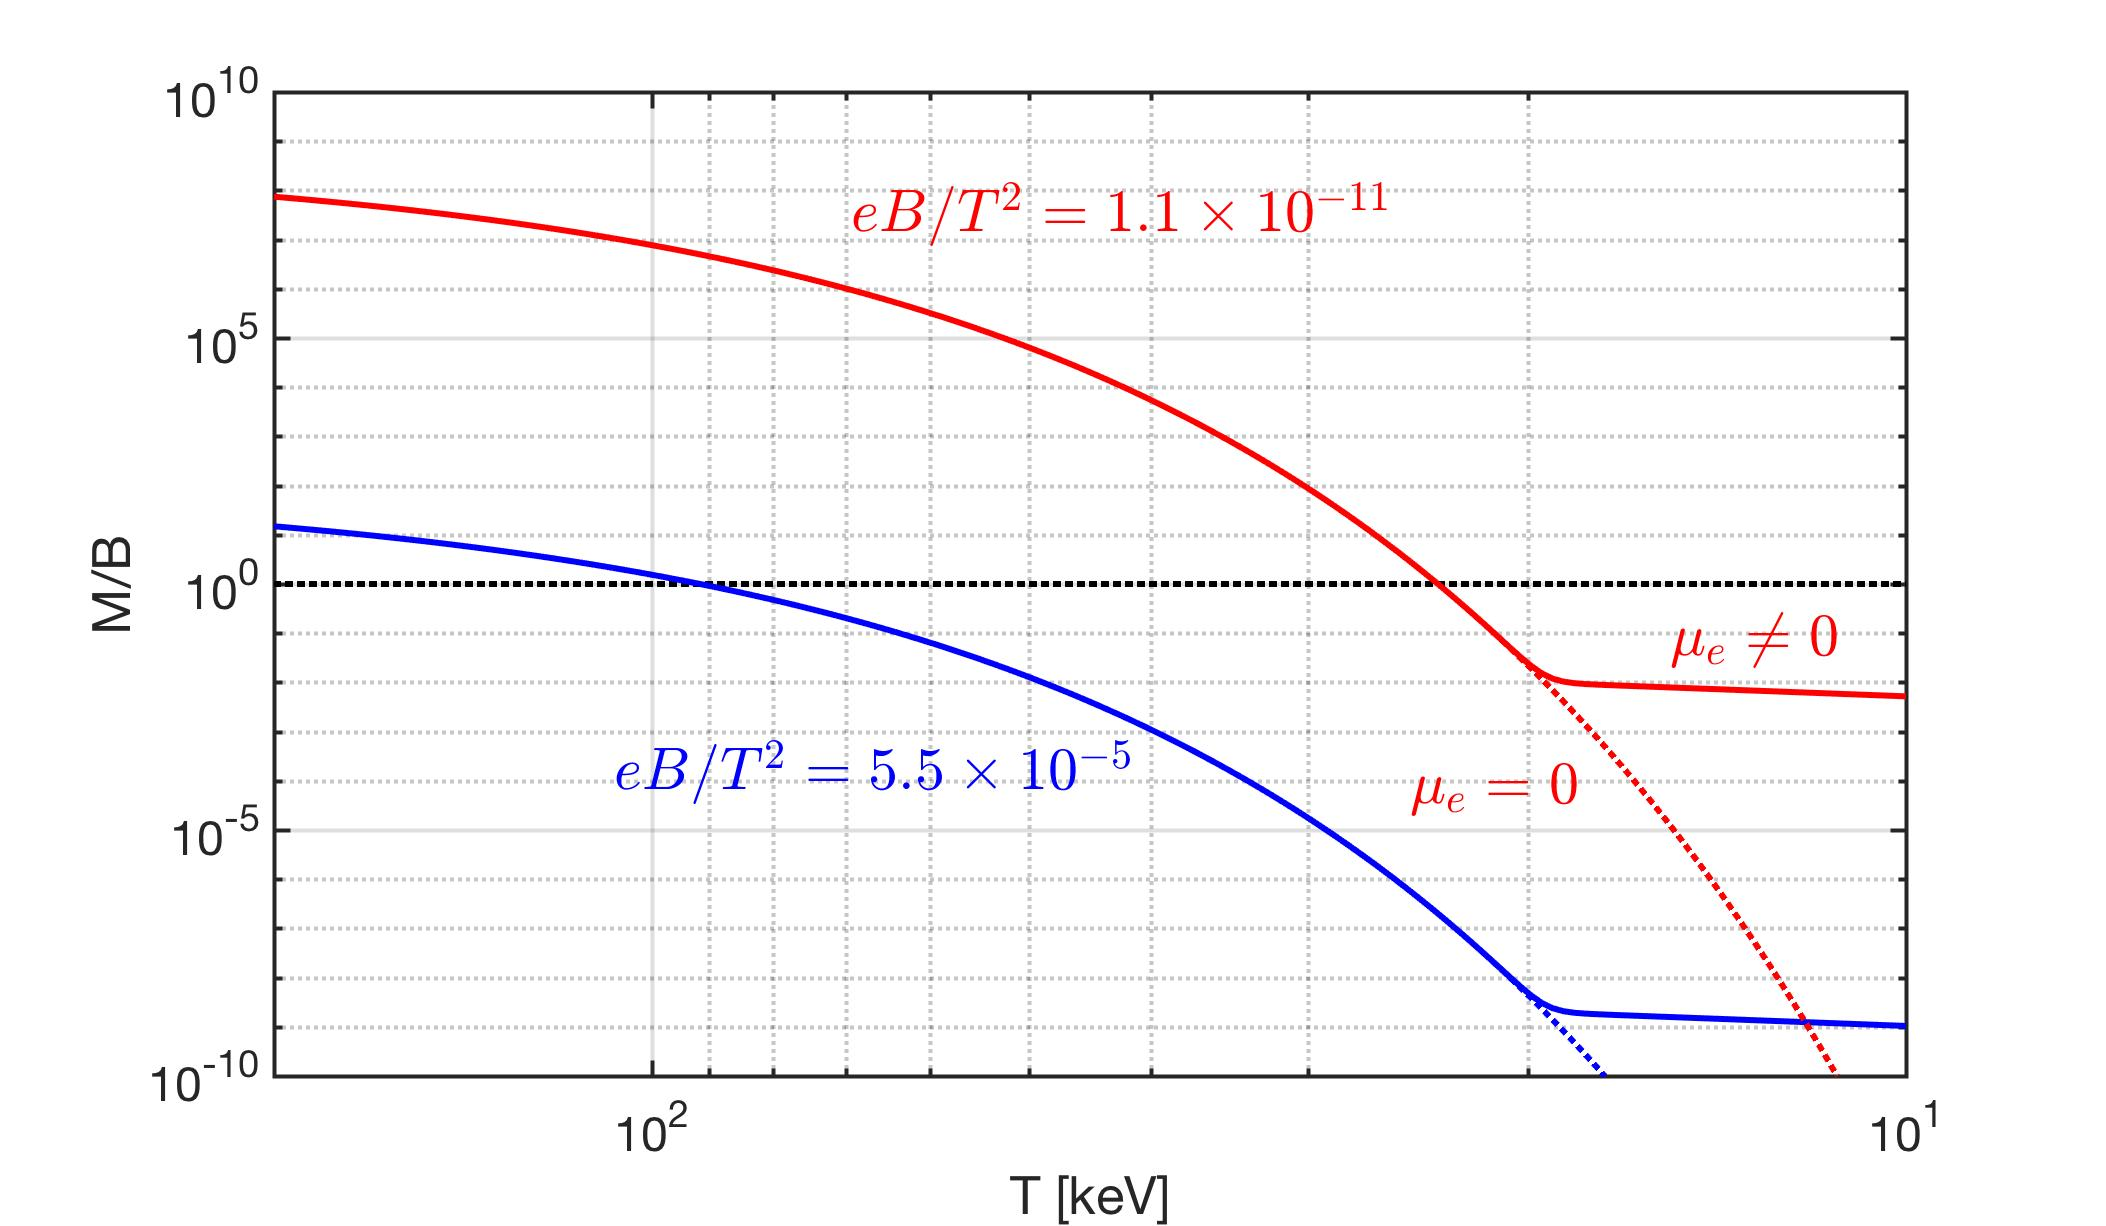
\includegraphics[width=\textwidth]{MagnetizationFinal_200keV.jpg}
\caption{The chemical potential $\eta_{e}/T$(upper) and magnetization $M/B$(lower) as a function of temperature $20<T<60$keV  for the case 2.  It shows that for giving $b_0$ we can find the temperature that $M/B>1$ in early universe.}
\label{Case2_fig} 
\end{figure}
%%%%%%%%%%%%%%%%%%%%%%%%%%%%%%%%%%%%%%%

\section{Summary}

%%%%%%%%%%%%%%%%%%%%%%%%%%%%%%%%%%%%%%%
\begin{itemize}
    \item {\xred Bibliography styles between Jeremey and us differ. Make homogeneous, probably go with BibTeX like Jeremey uses as it's cleaner as a separate file.}
\end{itemize}
\reftitle{References}
\begin{thebibliography}{99}

\bibitem{Fromerth:2012fe}
M.~J.~Fromerth, I.~Kuznetsova, L.~Labun, J.~Letessier and J.~Rafelski,
``From Quark-Gluon Universe to Neutrino Decoupling: 200 < T < 2MeV,''
Acta Phys. Polon. B \textbf{43}, no.12, 2261-2284 (2012)
doi:10.5506/APhysPolB.43.2261

\bibitem{Yang:2021bko}
C.~T.~Yang and J.~Rafelski,
``Cosmological strangeness abundance,''
Phys. Lett. B \textbf{827}, 136944 (2022)
doi:10.1016/j.physletb.2022.136944

\bibitem{Birrell:2012gg} 
J.~Birrell, Cheng~Tao~Yang, P.~Chen and J.~Rafelski,
\lq\lq Relic neutrinos: Physically consistent treatment of effective number of neutrinos and neutrino mass,\rq\rq
Phys.\ Rev.\ D {\bf 89}, 023008 (2014)
doi:10.1103/PhysRevD.89.023008
[arXiv:1212.6943 [astro-ph.CO]].

\bibitem{Chris:2023abc}
Christopher Grayson, C.~T.~Yang and J.~Rafelski,
``Electron-Positron Plasma in BBN epoch,'' (to be published).

\bibitem{Pitrou:2018cgg} 
C.~Pitrou, A.~Coc, J.~P.~Uzan and E.~Vangioni,
\lq\lq Precision big bang nucleosynthesis with improved Helium-4 predictions,\rq\rq\ 
arXiv:1801.08023 [astro-ph.CO], Phys. Rep. {\it in press} (2018)


\bibitem{Wang:2010px} 
B.~Wang, C.~A.~Bertulani and A.~B.~Balantekin,
\lq\lq Electron screening and its effects on Big-Bang nucleosynthesis, \rq\rq
Phys.\ Rev.\ C {\bf 83}, 018801 (2011)
doi:10.1103/PhysRevC.83.018801
[arXiv:1010.1565 [astro-ph.CO]].

\bibitem{Mangano:2005cc} 
G.~Mangano, G.~Miele, S.~Pastor, T.~Pinto, O.~Pisanti and P.~D.~Serpico,
\lq\lq Relic neutrino decoupling including flavor oscillations,\rq\rq\
Nucl.\ Phys.\ B {\bf 729}, 221 (2005)
doi:10.1016/j.nuclphysb.2005.09.041
[hep-ph/0506164].

\bibitem{Birrell:2014uka} 
 J.~Birrell, Cheng~Tao~Yang and J.~Rafelski,
\lq\lq Relic Neutrino Freeze-out: Dependence on Natural Constants,\rq\rq\
 Nucl.\ Phys.\ B {\bf 890}, 481 (2014)
 doi:10.1016/j.nuclphysb.2014.11.020
 [arXiv:1406.1759 [nucl-th]].


\bibitem{ParticleDataGroup:2022pth}
R.~L.~Workman \textit{et al.} [Particle Data Group],
``Review of Particle Physics,''
PTEP \textbf{2022}, 083C01 (2022)
doi:10.1093/ptep/ptac097

\bibitem{Kolb:1990vq} 
E.~W.~Kolb and M.~S.~Turner,
\emph{The Early Universe},
547 pp, Front.\ Phys.\ {\bf 69}, 1 (1990),
ISBN: 0201626748, 9780201626742

%\cite{Strickland:2012vu}
\bibitem{Strickland:2012vu}
M.~Strickland, V.~Dexheimer and D.~P.~Menezes,
``Bulk Properties of a Fermi Gas in a Magnetic Field,''
Phys. Rev. D \textbf{86} (2012), 125032
doi:10.1103/PhysRevD.86.125032
[arXiv:1209.3276 [nucl-th]].
%101 citations counted in INSPIRE as of 16 Mar 2023

%\cite{Steinmetz:2018ryf}
\bibitem{Steinmetz:2018ryf}
A.~Steinmetz, M.~Formanek and J.~Rafelski,
``Magnetic Dipole Moment in Relativistic Quantum Mechanics,''
Eur. Phys. J. A \textbf{55} (2019) no.3, 40
doi:10.1140/epja/i2019-12715-5
[arXiv:1811.06233 [hep-ph]].
%17 citations counted in INSPIRE as of 16 Mar 2023

%\cite{Rafelski:2022bsv}
\bibitem{Rafelski:2022bsv}
J.~Rafelski, S.~Evans and L.~Labun,
``Study of QED singular properties for variable gyromagnetic ratio $g\simeq 2$,''
[arXiv:2212.13165 [hep-th]].
%0 citations counted in INSPIRE as of 16 Mar 2023


%\cite{Fromerth:2012fe}
\bibitem{Fromerth:2012fe}
M.~J.~Fromerth, I.~Kuznetsova, L.~Labun, J.~Letessier and J.~Rafelski,
``From Quark-Gluon Universe to Neutrino Decoupling: 200 \ensuremath{<} T \ensuremath{<} 2MeV,''
Acta Phys. Polon. B \textbf{43}, no.12, 2261-2284 (2012)
doi:10.5506/APhysPolB.43.2261
[arXiv:1211.4297 [nucl-th]].
%17 citations counted in INSPIRE as of 17 Mar 2023

\bibitem{Birrell:2012gg}
J.~Birrell, C.~T.~Yang, P.~Chen and J.~Rafelski,
``Relic neutrinos: Physically consistent treatment of effective number of neutrinos and neutrino mass,''
Phys. Rev. D \textbf{89}, 023008 (2014)
doi:10.1103/PhysRevD.89.023008


\bibitem{Birrell:2014gea}
J.~Birrell, J.~Wilkening and J.~Rafelski,
``Boltzmann Equation Solver Adapted to Emergent Chemical Non-equilibrium,''
J. Comput. Phys. \textbf{281}, 896-916 (2015)
doi:10.1016/j.jcp.2014.10.056

\bibitem{Choquet-Bruhat:2009xil}
Y.~Choquet-Bruhat,
``General Relativity and the Einstein Equations,''
Oxford University Press, 2009,
ISBN 978-0-19-923072-3

\bibitem{Rafelski:2021aey}
J.~Rafelski and C.~T.~Yang,
``The muon abundance in the primordial Universe,''
Acta Phys. Polon. B \textbf{52}, 277 (2021)
doi:10.5506/APhysPolB.52.277

\bibitem{Kuznetsova:2008jt}
I.~Kuznetsova, D.~Habs and J.~Rafelski,
``Pion and muon production in e-, e+, gamma plasma,''
Phys. Rev. D \textbf{78}, 014027 (2008)
doi:10.1103/PhysRevD.78.014027

%\bibitem{Aksenov:2007}
%A. G. Aksenov, R. Ruffini, and G. V. Vereshchagin
%``Thermalization of Nonequilibrium Electron-Positron-Photon Plasmas,''
%Phys.\ Rev.\ Lett.\ \textbf{99}, 125003 (2007) 
%doi: 10.1103/PhysRevLett.99.125003

%\bibitem{Aksenov:2010}
%A. G. Aksenov, R. Ruffini, and G. V. Vereshchagin
%``Pair plasma relaxation time scales''
%Phys.\ Rev.\ E \textbf{81}, 046401 (2010)
%doi: 10.1103/PhysRevE.81.046401
\end{thebibliography}

%%%%%%%%%%%%%%%%%%%%%%%%%%%%%%%%%%%%%%%
\end{document}
